% https://github.com/martinhelso/MathDept


\documentclass[UKenglish]{beamer}


\usetheme[NoLogo]{MathDept}


\usepackage[utf8]{inputenx} % For æ, ø, å
\usepackage{babel}          % Automatic translations
\usepackage{csquotes}       % Quotation marks
\usepackage{microtype}      % Improved typography
\usepackage{amssymb}        % Mathematical symbols
\usepackage{mathtools}      % Mathematical symbols
\usepackage[absolute, overlay]{textpos} % Arbitrary placement
\setlength{\TPHorizModule}{\paperwidth} % Textpos units
\setlength{\TPVertModule}{\paperheight} % Textpos units
\usepackage{tikz}
\usepackage{diagbox}
\usetikzlibrary{overlay-beamer-styles}  % Overlay effects for TikZ


\author{William Hirst}
\title[Supervised Learning in HEP]{Application of Supervised Machine Learning to the Search for New Physics in ATLAS data}
\subtitle{A Study of Ordinary Dense, Parameterized and Ensemble Networks and their Application to High Energy Physics}


\begin{document}


\begin{frame}{Outline}
    \tableofcontents
\end{frame}


\section{Introduction $\&$ Motivation}
\begin{frame}{Outline}
    \tableofcontents[currentsection]
\end{frame}

\begin{frame}{Why apply machine learning to HEP problems?}
    \begin{itemize}
        \item The standard model of particle physics is one of the most 
              successful theories of all time
        \item Some aspects of the universe are currently not described by the 
              standard model 
        \begin{itemize}
            \item Neutrino masses 
            \item Hierarchy problem 
            \item Energy-matter density in the universe
        \end{itemize}
        \item To precisely test extensions of the standard model we produce 
        progressively larger amounts of data
        \item Upholding the quality of analysis demands advanced tools
        \begin{itemize}
            \item Machine learning
        \end{itemize}
    \end{itemize}
\end{frame}


\begin{frame}{How do we search for new physics?}
    \begin{textblock}{1}(0.515,0.585)
        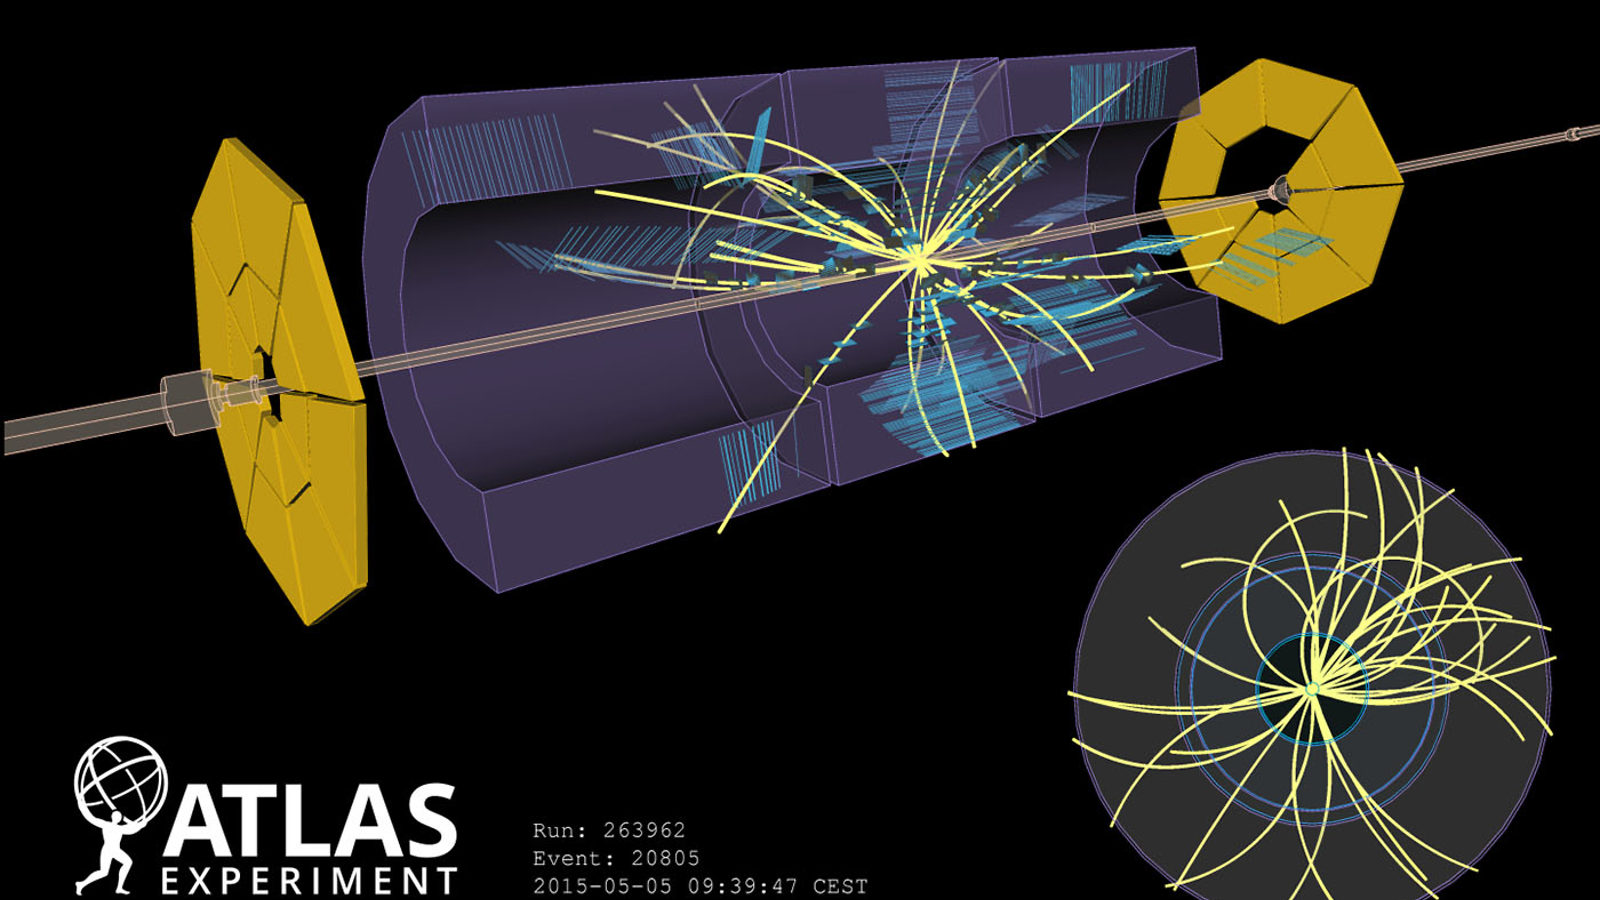
\includegraphics[width=0.475\textwidth]{figures/Collisions.jpeg}
    \end{textblock}
    \begin{itemize}
        \item Two data sets 
        \begin{itemize}
            \item Theory: Simulated based on Standard model physics 
            \item Experiment: Proton-proton collisions measured in particle detectors
        \end{itemize}
        \item Data sets include information regarding collisions (momentum and mass of particles, collision angle etc.)
        \item Compare theory with experiment 
        \begin{itemize}
            \item Match: Standard model adequately explain collision
            \item Deviations: New physics, or statistical fluctuations 
        \end{itemize}
        \item Create search region
        \begin{itemize}
            \item Traditional: Cut-and-Count
        \end{itemize}
        \item Measure deviation in \\ significance, Z 
        \begin{itemize}
            \item $Z\approx \frac{n_{obs} - bkg}{\sqrt{bkg}} = \frac{signal}{\sqrt{background}}$
        \end{itemize}
    \end{itemize}

\end{frame}
\begin{frame}
    \centering
    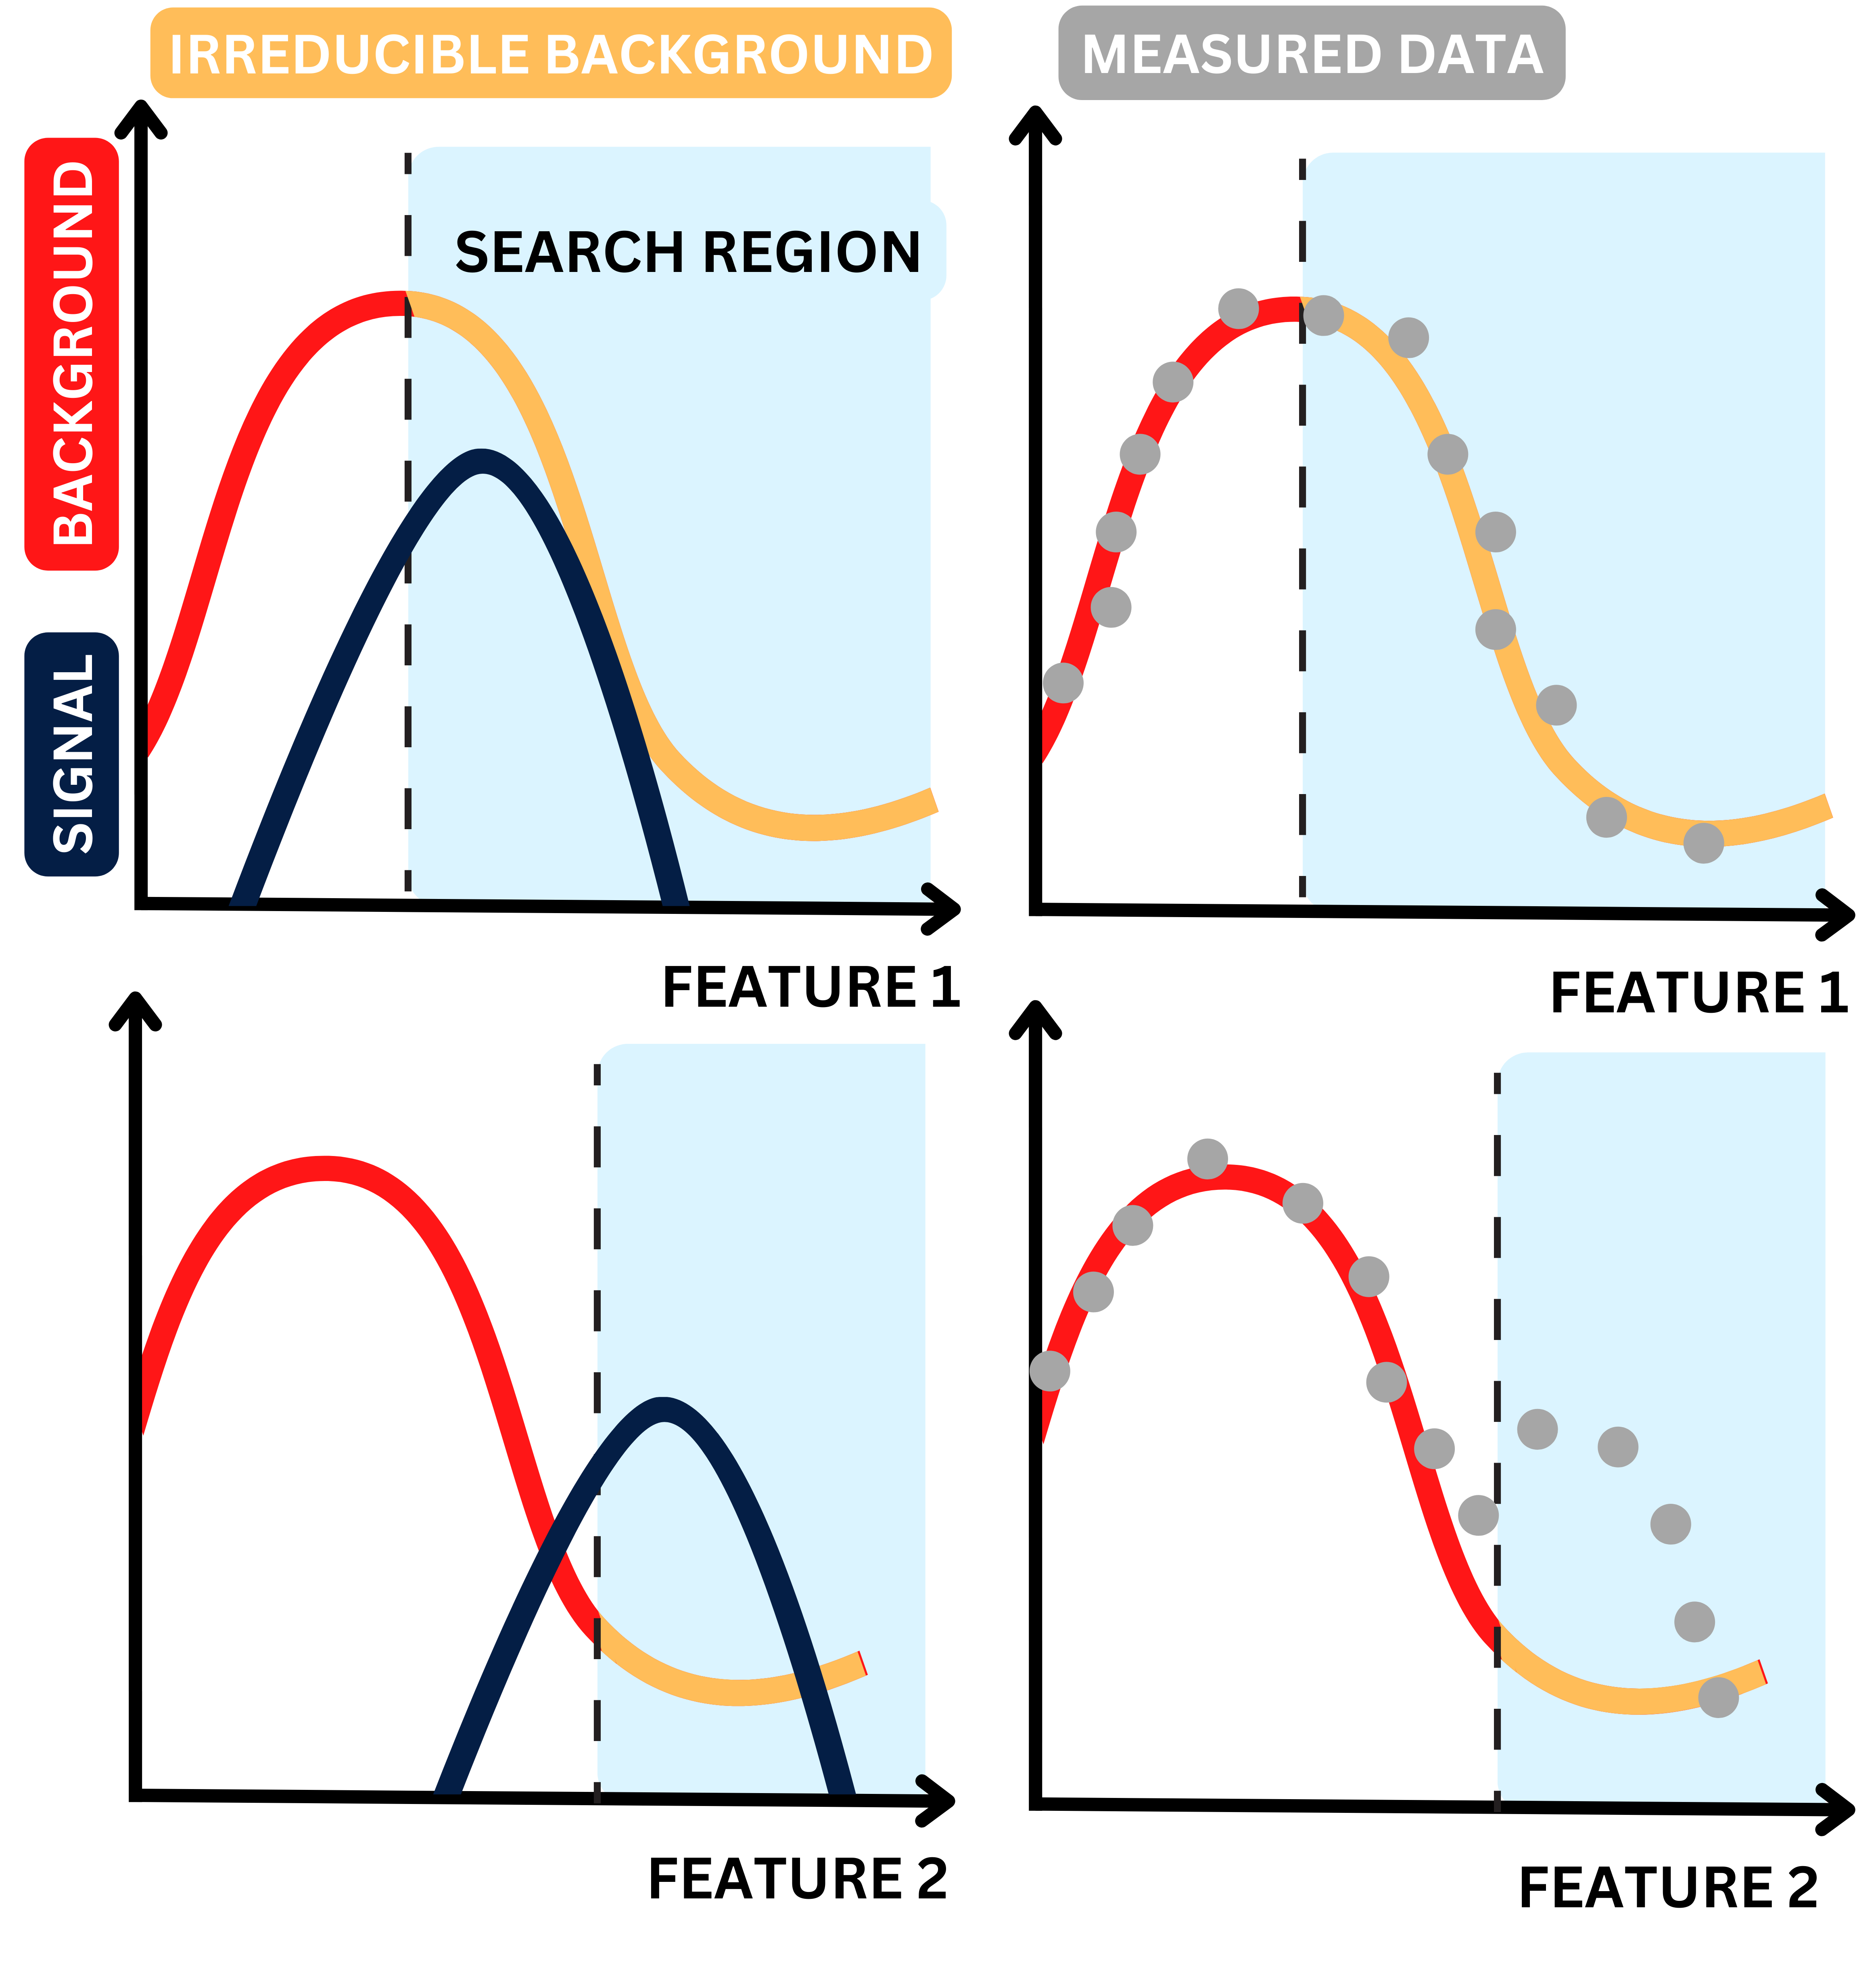
\includegraphics[width = 0.65\textwidth]{figures/DataComp.png}
\end{frame}
\begin{frame}{The search}
    \begin{itemize}
        \item Study application of supervised learning as it searches for SUSY signal 
        \begin{itemize}
            \item Chargino-neutralino production
            \item 2 free parameters: masses of the chargino and neutralino
        \end{itemize}
        \item Measure sensitivity of an analysis 
        \begin{itemize}
            \item Expected significance
            \item How many collisions do we expect to find in search region?
        \end{itemize} 
    \end{itemize}
    % \vfill
    \centering
    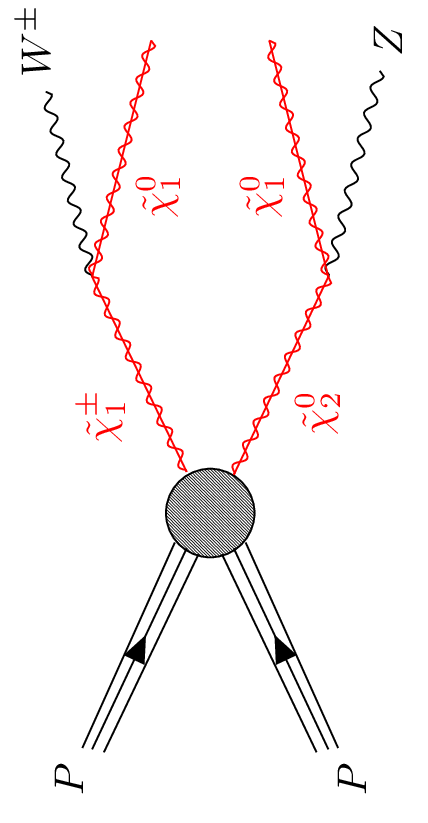
\includegraphics[width=0.3\textwidth, angle = -90]{figures/WZSignal.png}
\end{frame}

\begin{frame}{This thesis}
    \begin{center}
        \emph{Shed some light on the application of supervised learning in HEP by 
        experimenting and studying a set of ML methods as they search for a set of SUSY signals.}
    \end{center}
    \vspace{0.5cm}
    \begin{enumerate}
        \item Study individual attributes of a set of supervised methods 
        \item Compare expected sensitivity between methods on a subset of data
        \item Attempt to increase sensitivity via feature reduction (PCA)
        \item Compare the expected limits achieved by best performing methods 
              to previous ATLAS analysis
    \end{enumerate}
\end{frame}

\section{The Implementation}
\begin{frame}{Outline}
    \tableofcontents[currentsection]
\end{frame}

\begin{frame}{A summary of the applied methods}
    \emph{Three} neural network variants
    \begin{itemize}
        \item Ordinary dense neural network
        \item Ensemble networks utilizing Local-Winner-Takes-All (LWTA) layers
        \item Parameterized neural networks (PNN)
    \end{itemize}
    \emph{One} boosted decision tree method
    \begin{itemize}
        \item XGBoost using default settings
    \end{itemize}
    \begin{textblock}{1}(0.,0.55)
        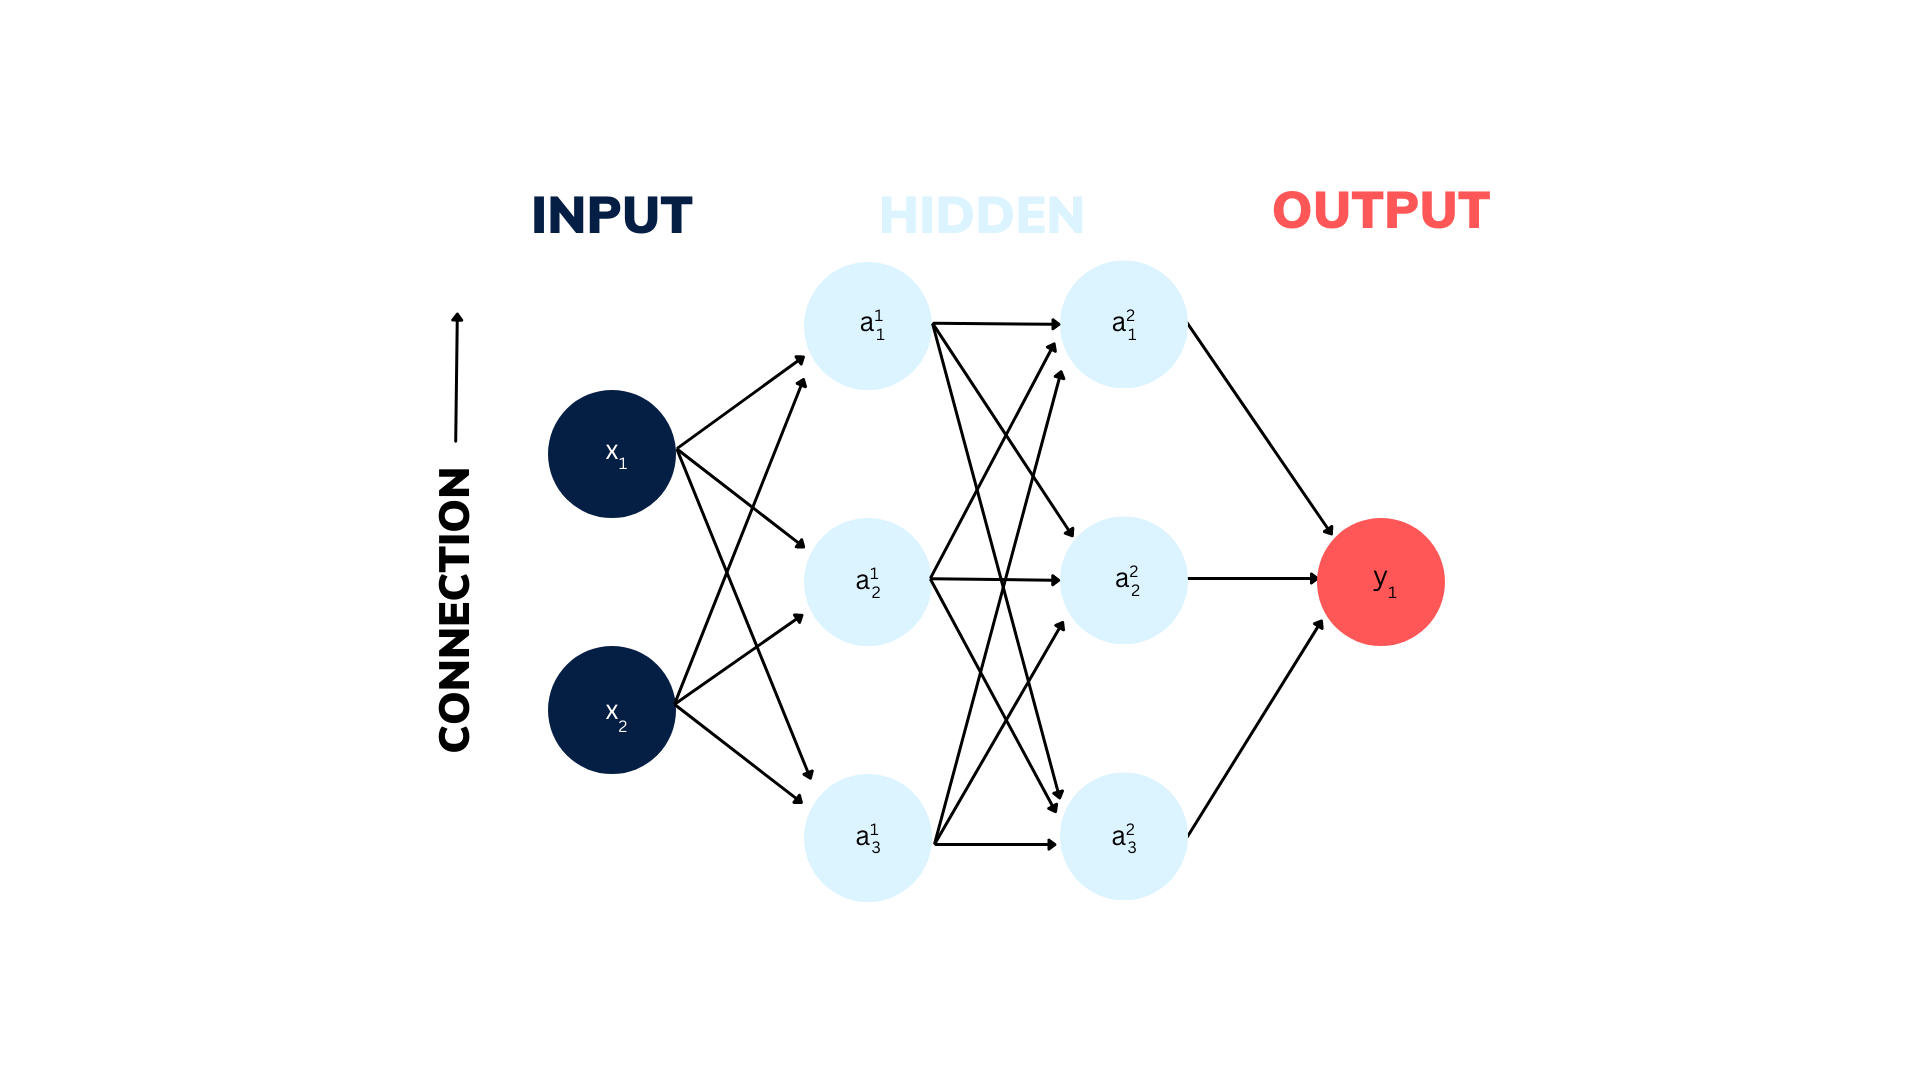
\includegraphics[width=0.525\textwidth]{figures/Input_labels.png}
    \end{textblock}
    \begin{textblock}{1}(.5,0.575)
        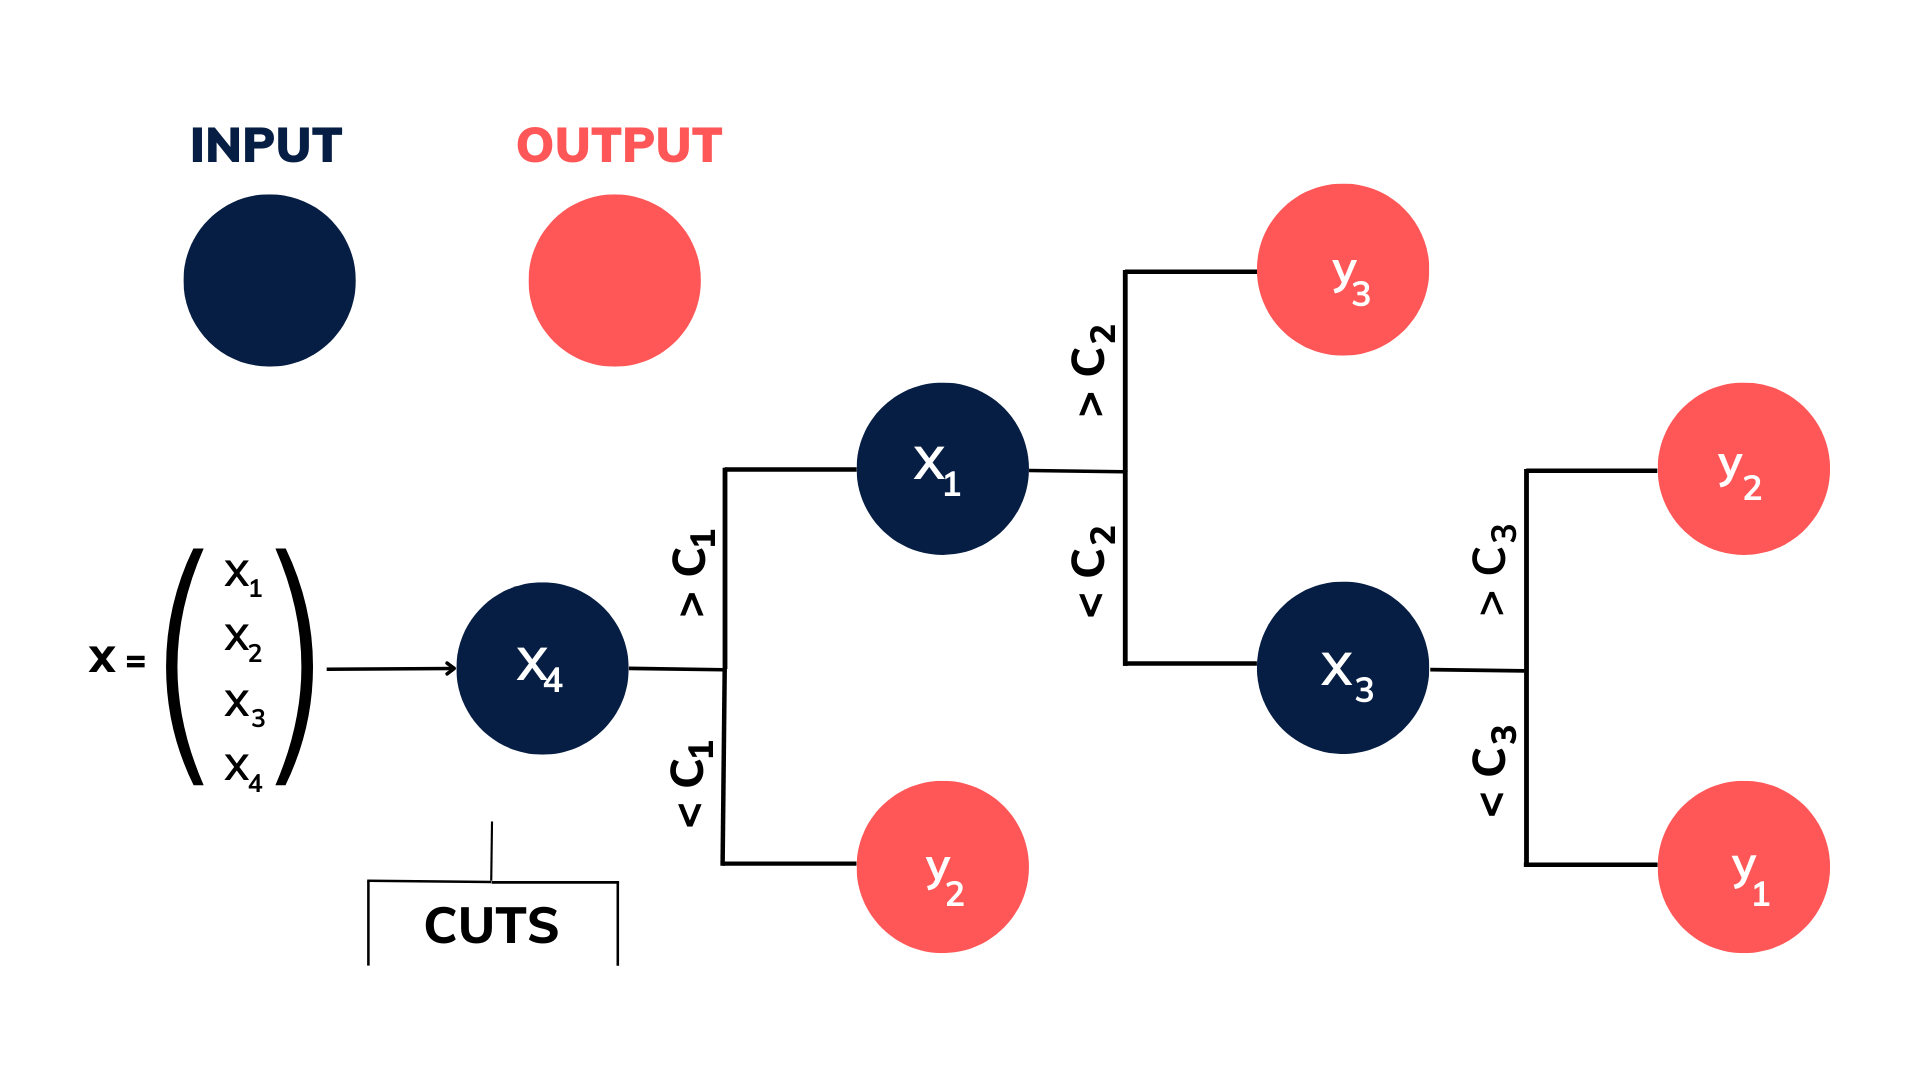
\includegraphics[width=0.435\textwidth]{figures/DT.png}
    \end{textblock}
\end{frame}

\begin{frame}{Training strategy}
    \begin{itemize}
        \item Train using simulated data 
        \item Objective: Classify standard model background as 0, and SUSY signal as 1
        \item $80\%$ training and $20\%$ validation 
        \item Early stopping criteria
        \begin{itemize}
            \item Train as long as performance on validation set improves 
            \item Patience 10 epochs
            \item Reset weights to best epoch
        \end{itemize}
    \end{itemize}
\end{frame}

\begin{frame}{Mass combinations of the chargino-neutralino pair}
    \begin{textblock}{1}(-0.02, 0.2)
        \begin{itemize}
            \item Full signal grid
            \begin{itemize}
                \item 89 mass\\ combinations
            \end{itemize}
            \item Original signal set: \\white corners
            \begin{itemize}
                \item 30 mass \\combinations
            \end{itemize}
            \item The smaller the \\masses,
                  the larger\\ the contribution            
        \end{itemize}
    \end{textblock}
    \begin{textblock}{1.0}(0.35,0.175)
        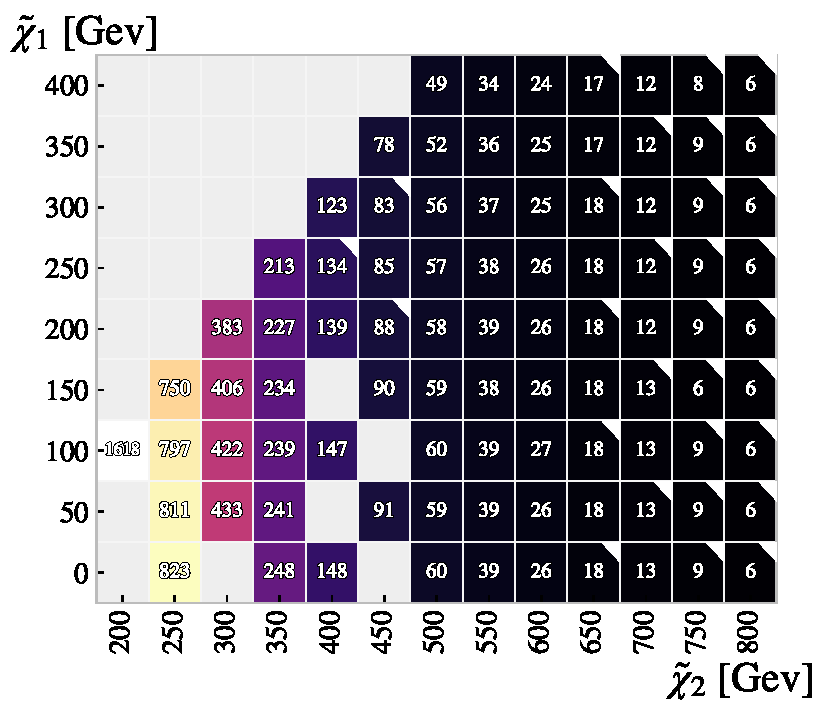
\includegraphics[width=0.65\textwidth]{figures/Signal/NrSignalEvents.pdf}
    \end{textblock}
\end{frame}



\section{Methods $\&$ Results}
\begin{frame}{Outline}
    \tableofcontents[currentsection]
\end{frame}


\begin{frame}{Boosted decision trees - XGBoost}
    \begin{textblock}{1}(0.35, 0.15)
        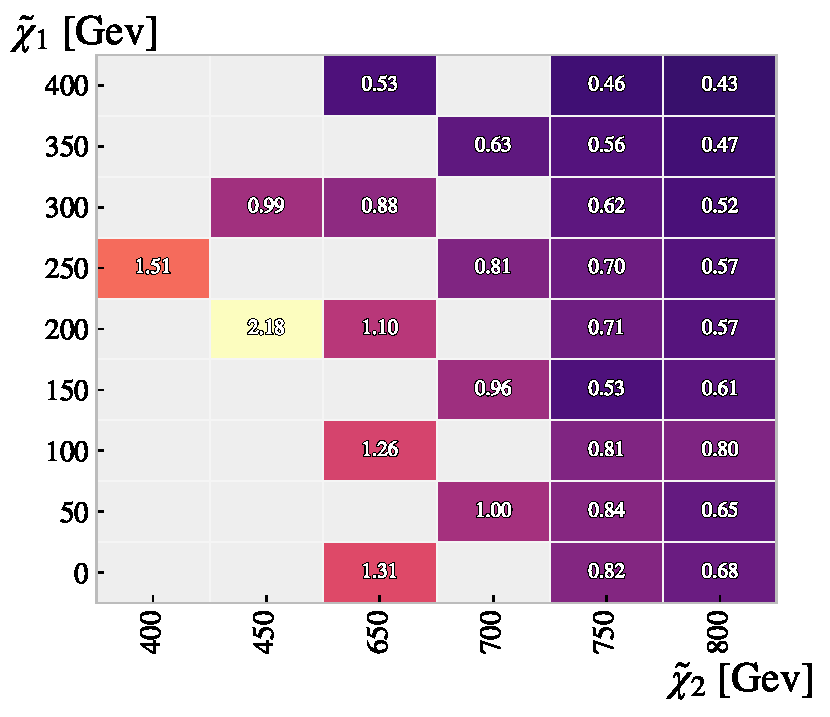
\includegraphics[width=0.65\textwidth]{figures/grids/XGBGridSig.pdf}    
    \end{textblock}
    \begin{textblock}{1}(-0.01, 0.2)
        \begin{itemize}
            \item Used as benchmark
            \item Minimal time spent\\ tuning BDT
            \item Trained on original \\ signal set
            \item Displayed better\\ performance on lower \\masses  
        \end{itemize}
    \end{textblock}
\end{frame}

% \begin{frame}{Sensitivity grid}
%     \vfill
%     \begin{center}
%         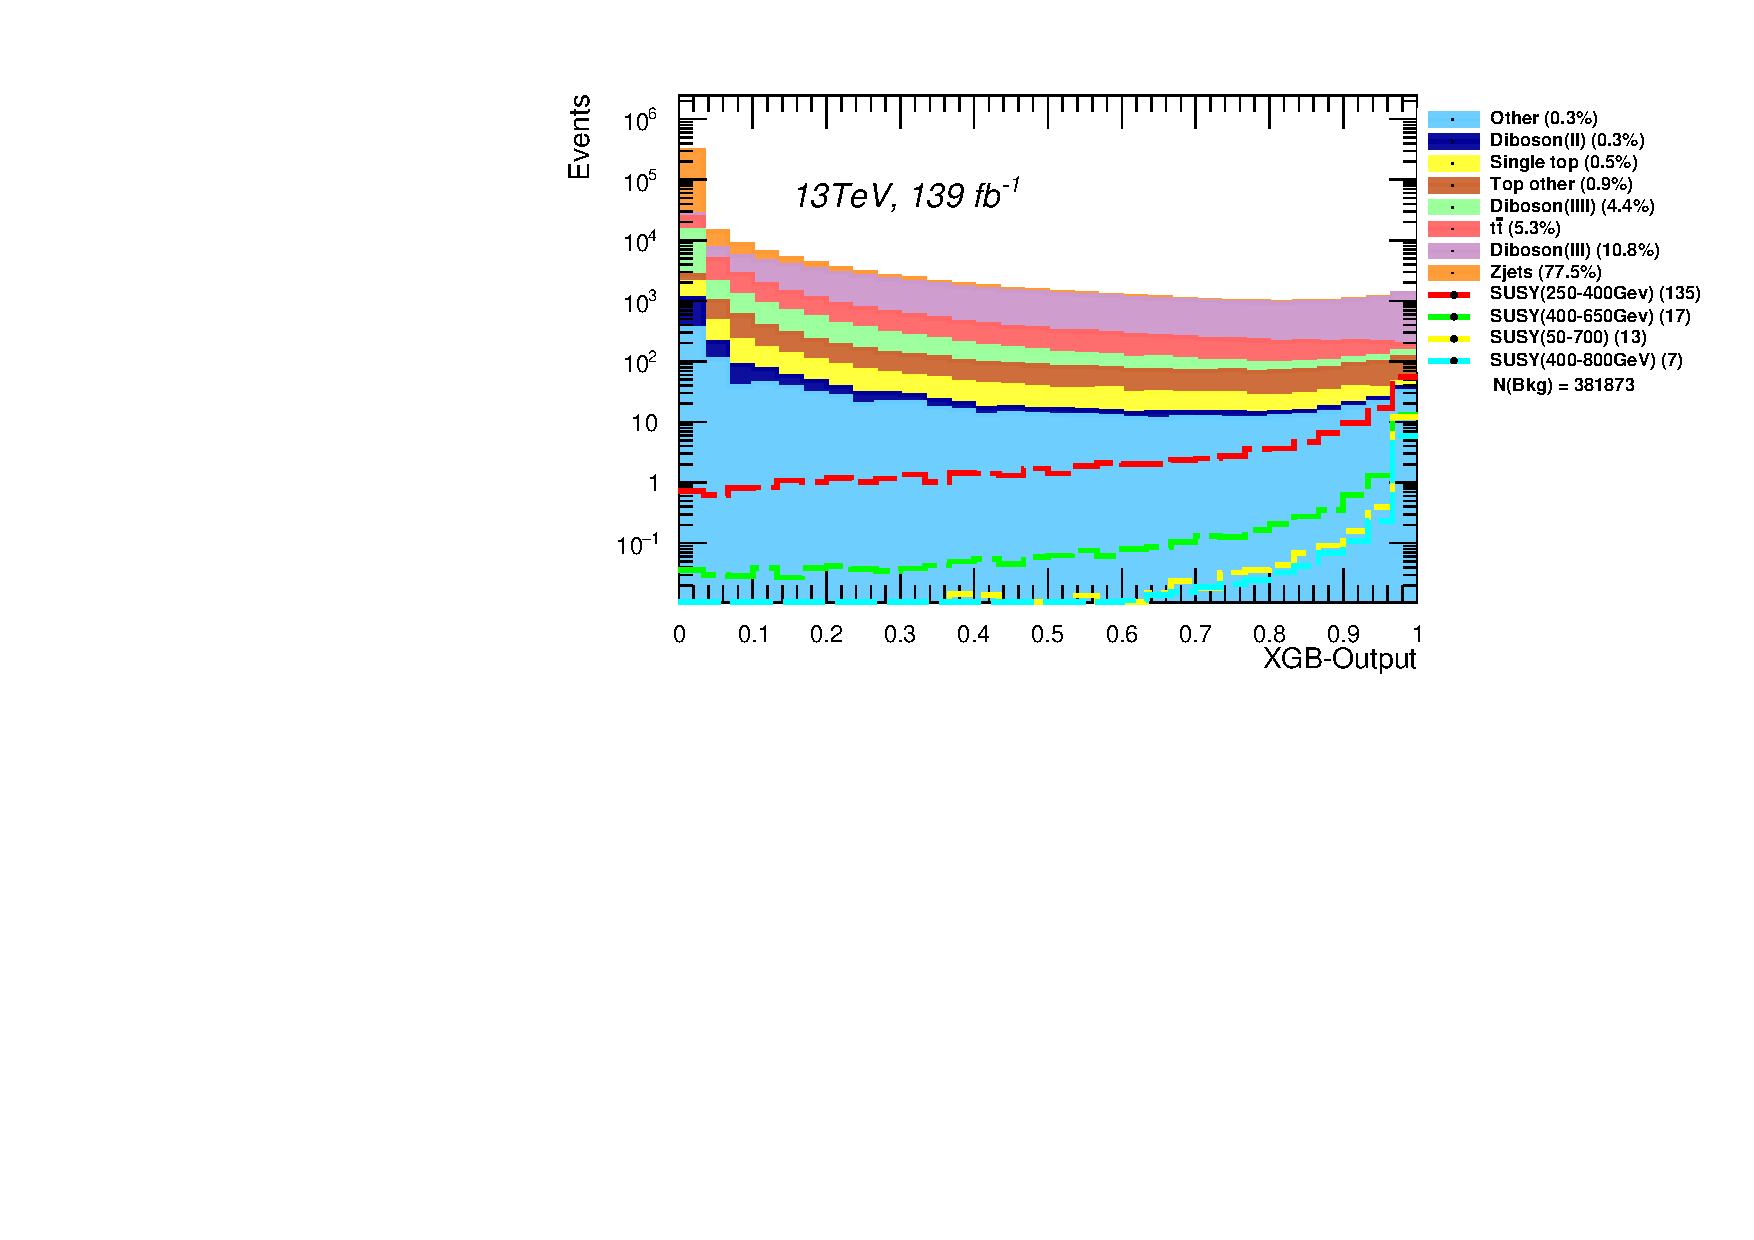
\includegraphics[width = 0.475\textwidth]{figures/dists/xgbDist.pdf}
%         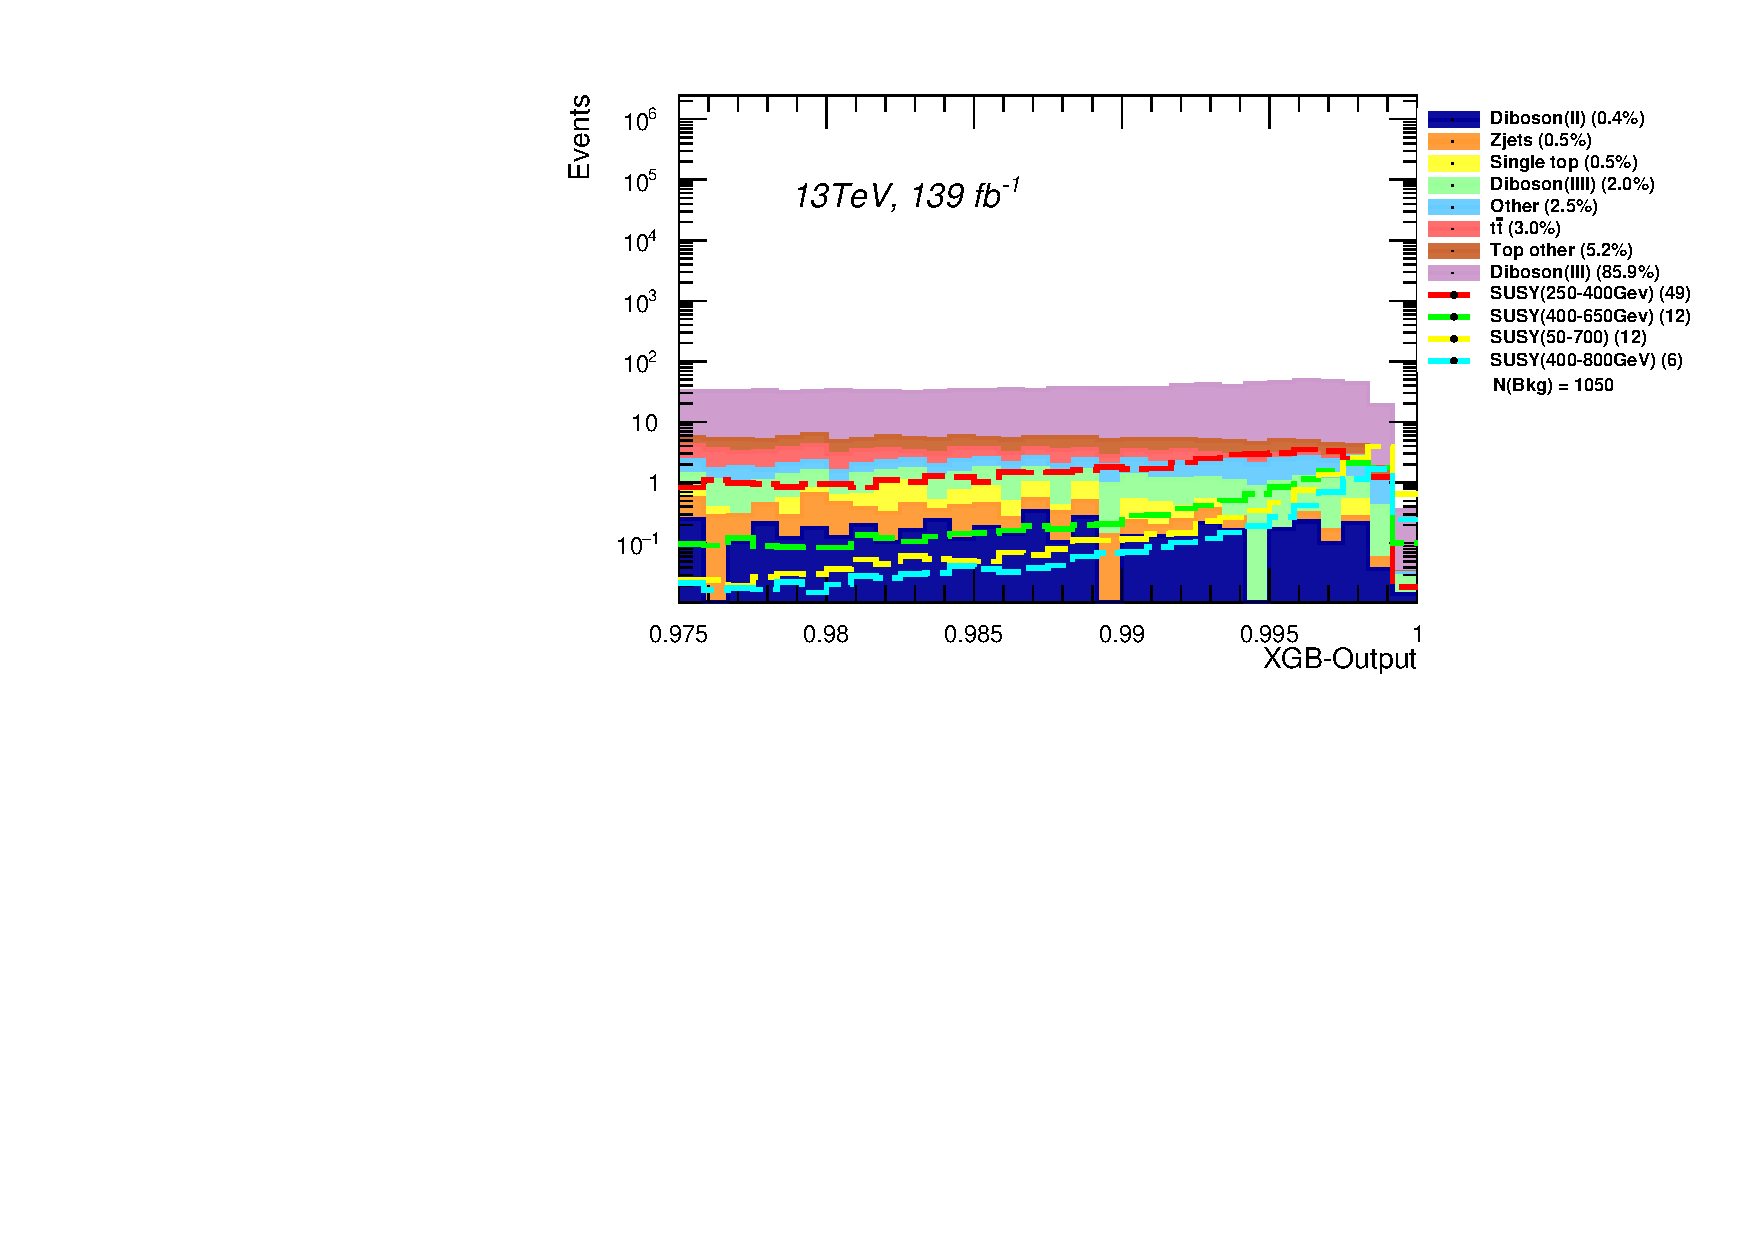
\includegraphics[width = 0.475\textwidth]{figures/dists/xgbDist_C7.pdf}
%     \end{center}
% \end{frame}

\begin{frame}{Ordinary dense neural network}
    \vfill
    \centering
    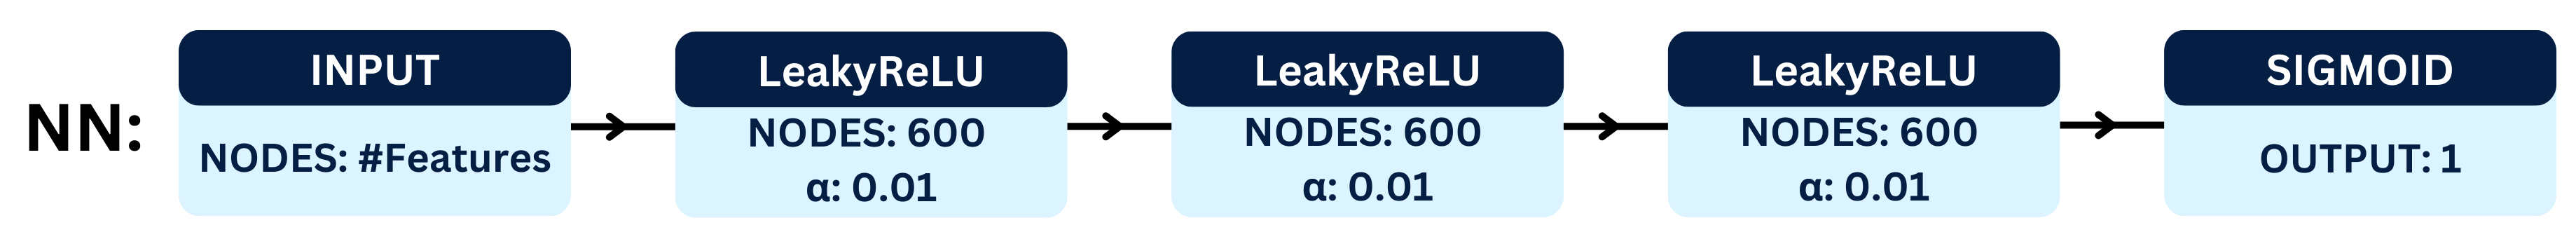
\includegraphics[width = 0.98\textwidth]{figures/NN.png}
\end{frame}
\begin{frame}{Compare one-mass approach to several-masses approach}
    \vfill
    \begin{center}
        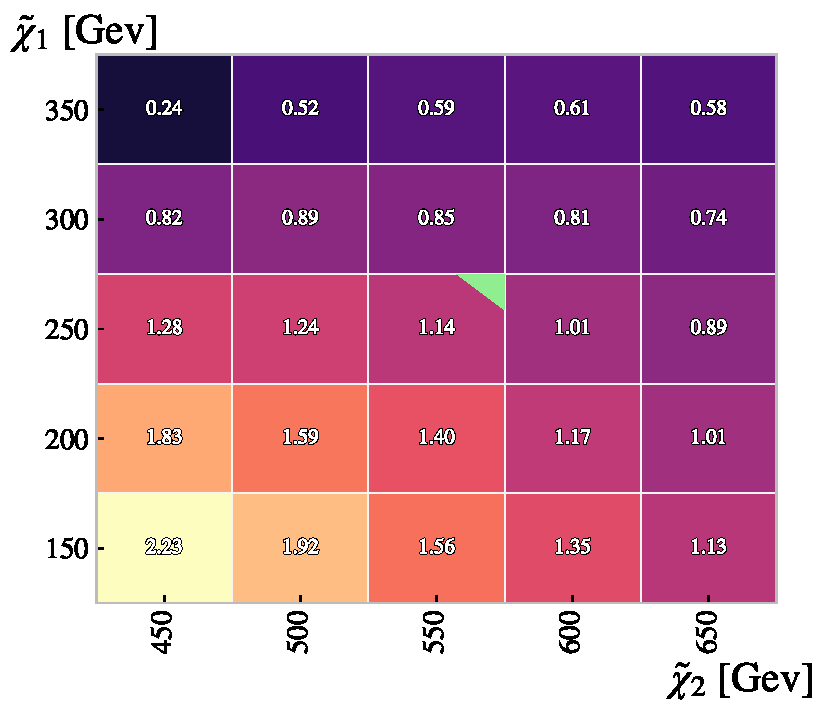
\includegraphics[width = 0.475\textwidth]{figures/grids/NN_OneMass_InterpolationGridSig.pdf}
        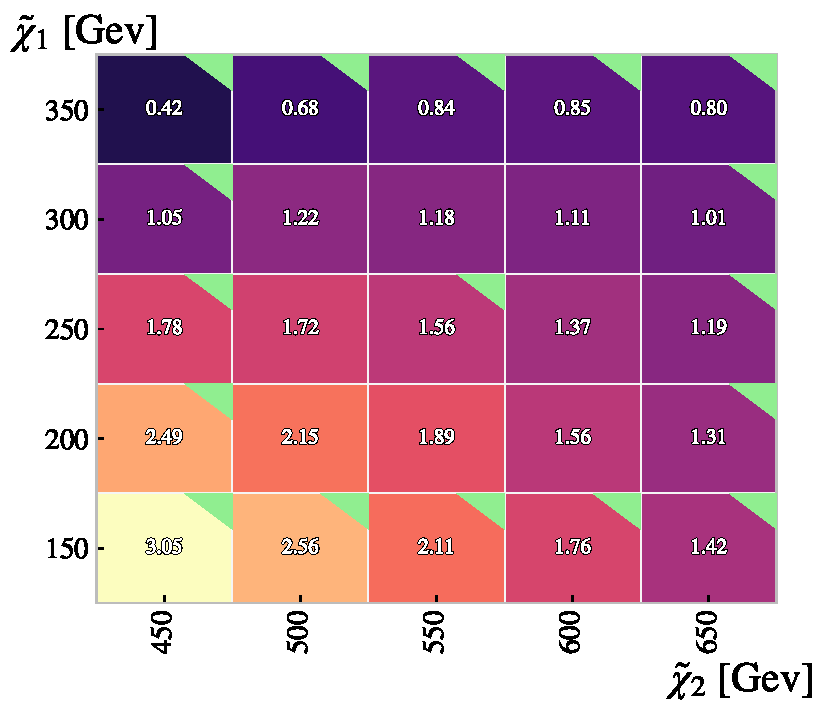
\includegraphics[width = 0.475\textwidth]{figures/grids/NN_InterpolationGridSig.pdf}
    \end{center}
\end{frame}


\begin{frame}{Parameterized neural network}
    \begin{itemize}
        \item For diverse data set, $X$, dependent on a parameter, $X(\theta)$
        \begin{itemize}
            \item Classical approach: One model for each parameter
            \item PNN approach: Include $\theta$ as feature in feature set
        \end{itemize}
        \item Signal events using masses $\{A,B\}_{GeV}$ to generate 
        event during simulation will include the parameters A and B
        in feature set
        \item Background assigned \\
        parameters randomly \\
        using same distribution\\ 
        as signal
        \item Motivation
        \begin{itemize}
            \item Network will \\
            associate parameters\\
            with trends in the \\
            data
        \end{itemize}
        \begin{textblock}{0.8}(0.45, 0.45)
            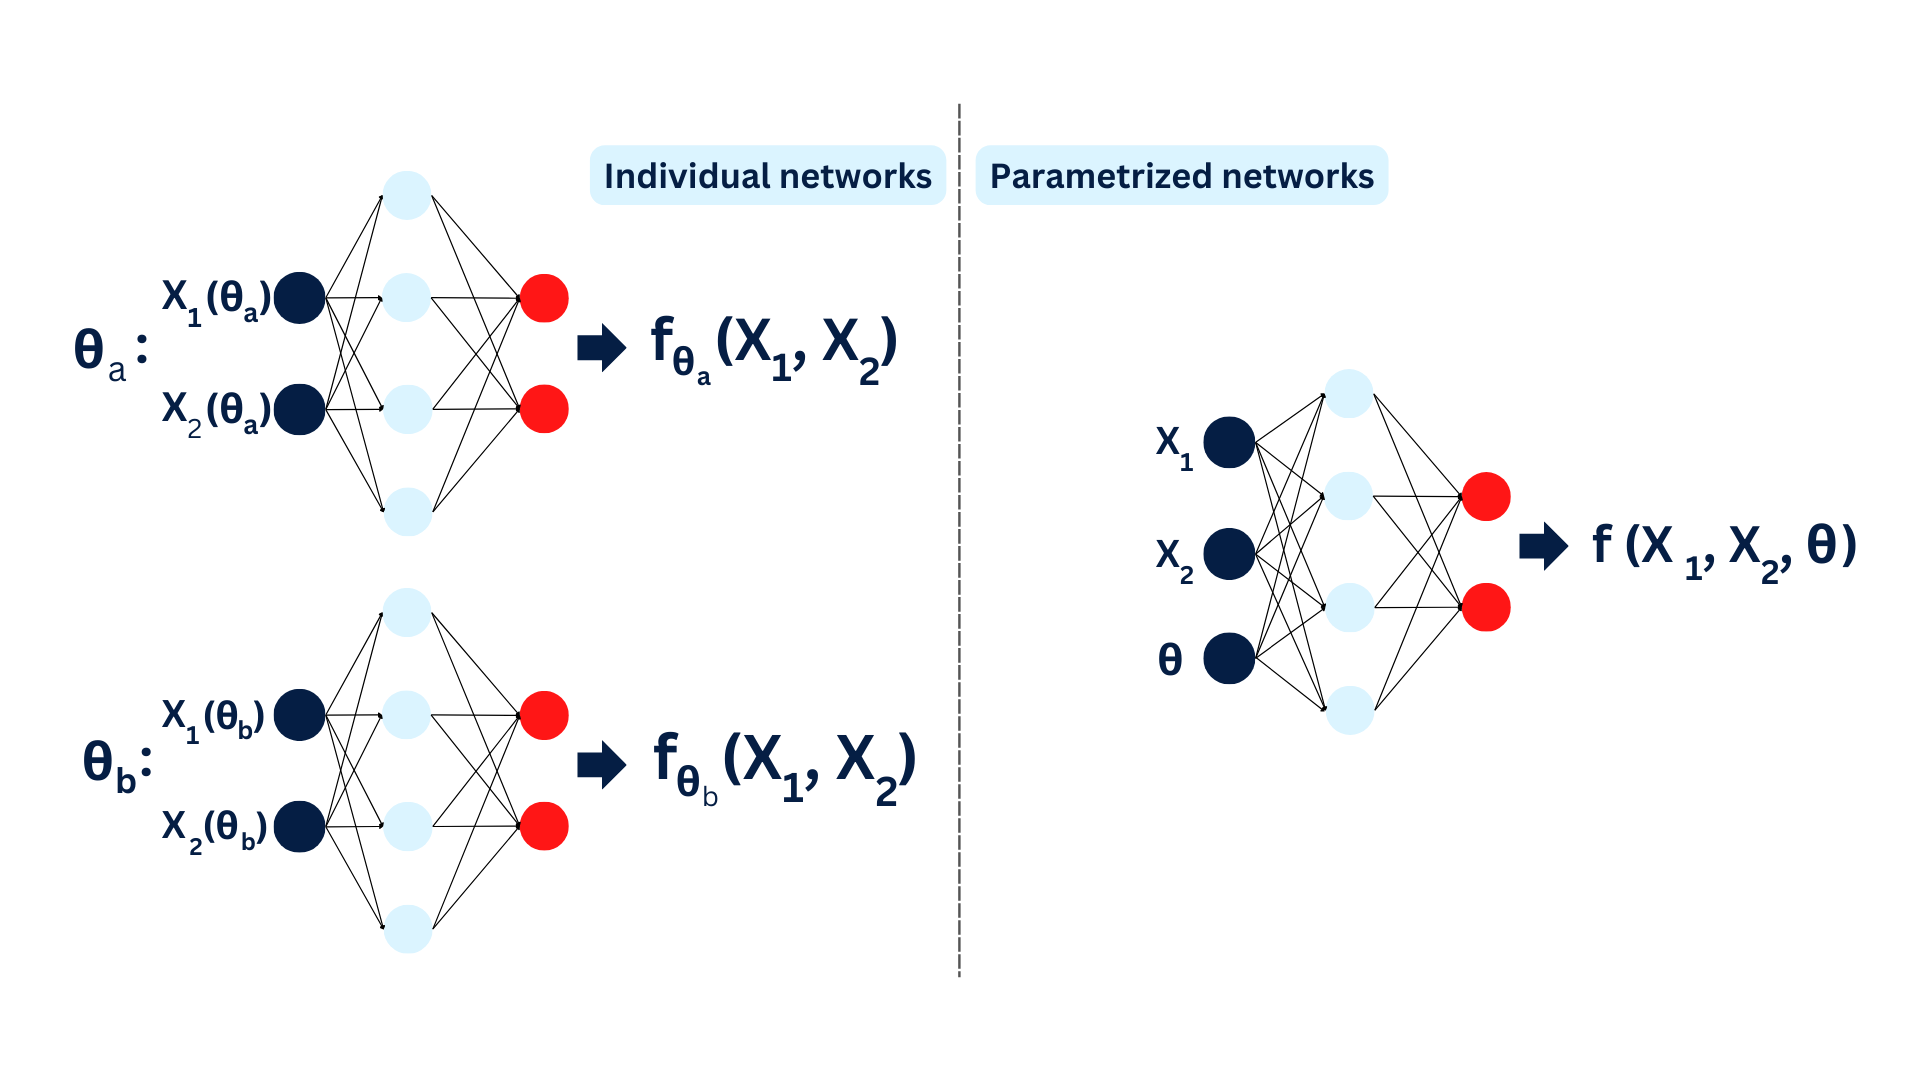
\includegraphics[width = 0.7\textwidth]{figures/PNN.png}
        \end{textblock}
    \end{itemize}
\end{frame}
\begin{frame}{PNN architecture}
    \vfill
    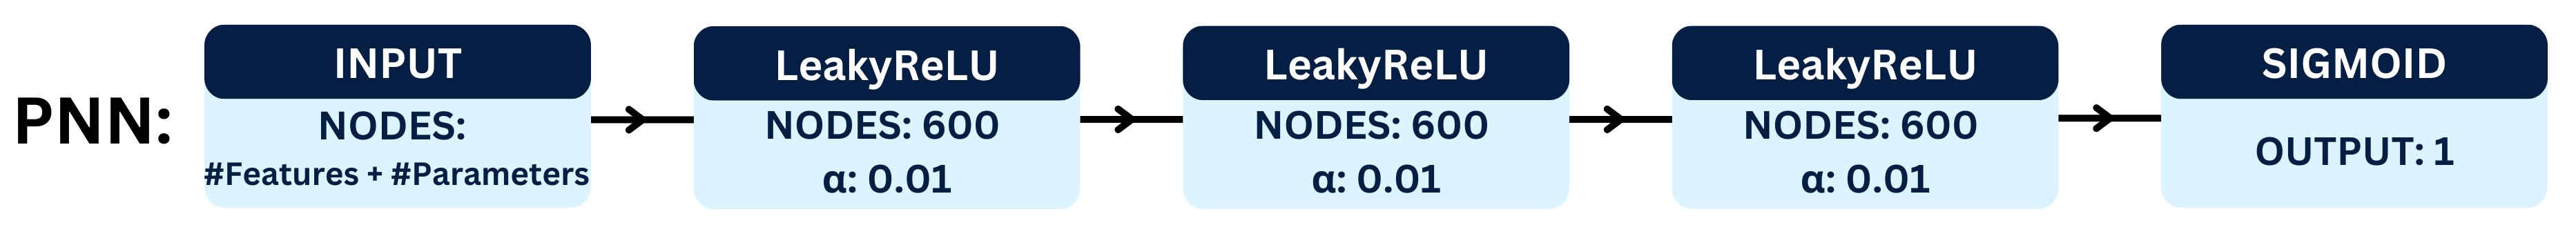
\includegraphics[width = 0.98\textwidth]{figures/PNNArch.png}
\end{frame}
\begin{frame}{Study the effect of the parameters in the PNN}
    \begin{itemize}
        \item Study if the parameters effect the training as intended
        \item Test: Manually assign all the events, both background and 
        signal, the same parameters (mass combinations) thereby assigning
        most of the signal the wrong parameters
        \item Hypothesis: PNN performs better when events are assigned correct
        parameters 
        \item First test: All events are given parameters $\{50,250\}_{GeV}$
        \item Second test: All events are given parameters $\{200,300\}_{GeV}$
    \end{itemize}
    \begin{table}
        \tiny
        \centering
        $
        \begin{array}{cccccc}
            \hline \text { \diagbox{\textbf{Parameters}}{\textbf{Channel}} }  & \text {$(50,250)$} & \text {$(100,200)$} & \text {$(150,300)$} & \text {$(200,300)$} & \text {$(Background)$} \\
            \hline \text {$(50,250)$}   & \text { $\bf{80.8}\%$ } & \text { $45.8\%$ } & \text { $\bf{77.5}\%$ } & \text { $50.1\%$ } & \text { $2.4\%$ }  \\
            \text {$(200,300)$}   & \text { $77.3\%$ } & \text { $\bf{54.6}\%$ } & \text { $76.3\%$ } & \text { $\bf{59.0}\%$ } & \text { $\bf{2.7}\%$ }\\
            \hline
        \end{array}
        $
    \end{table}
\end{frame}

\begin{frame}{Ensemble methods - LWTA}
    \begin{itemize}
        \item Dropout
        \item What is LWTA?
        \item Competing nodes - Units
        \item Encode information in pattern specific pathways
    \end{itemize}    
    \begin{textblock}{0.58}(0.2, 0.365)
        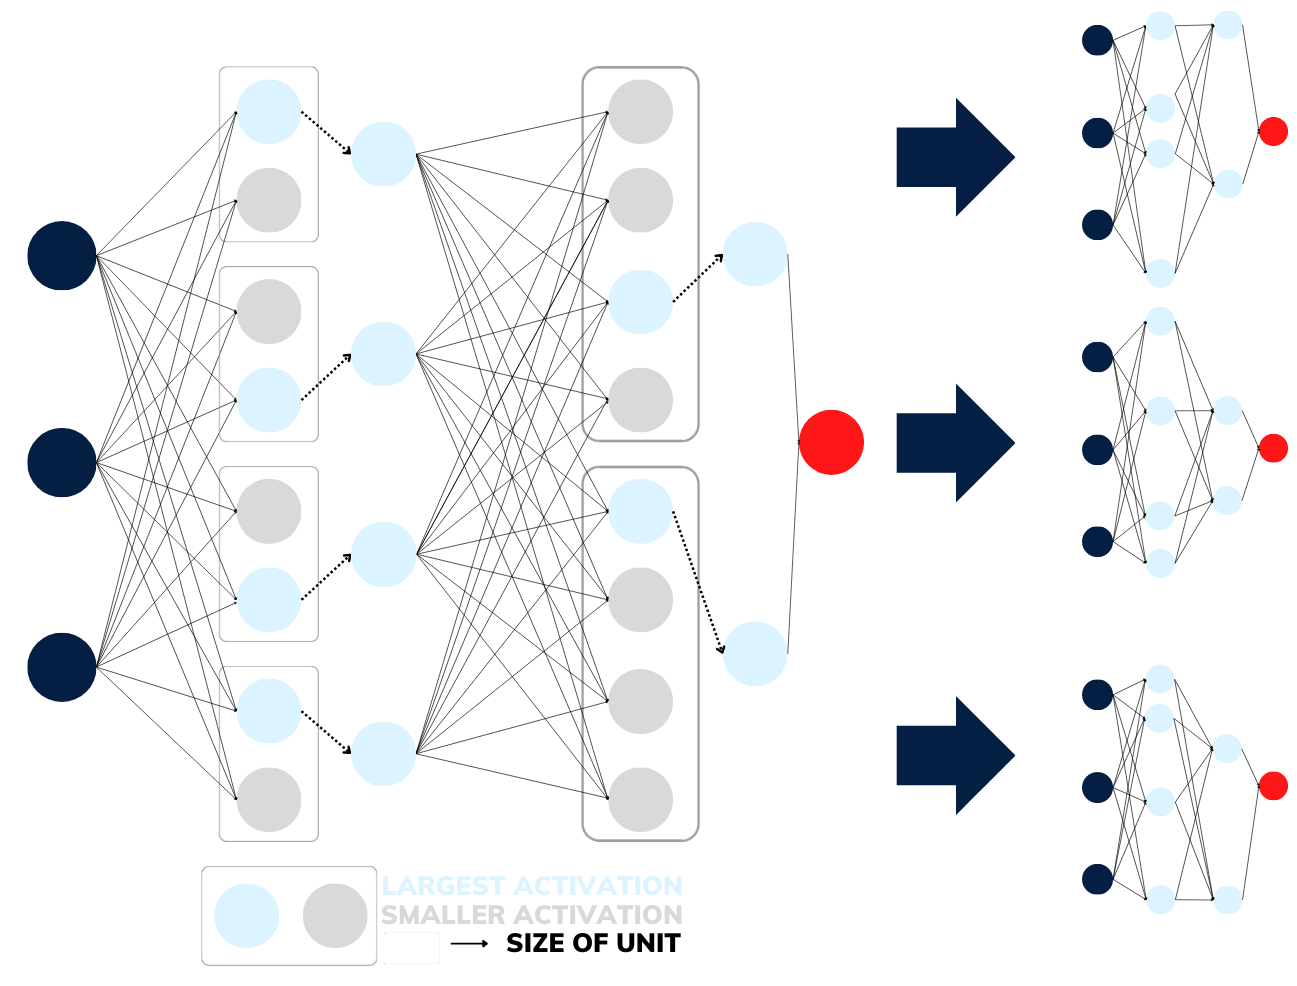
\includegraphics[width = \textwidth]{figures/Max_out}
    \end{textblock}
\end{frame}

\begin{frame}{Channel-Out, SCO and Maxout}
    \vspace{0.5cm}
    \center
        \begin{table}
            $
            \begin{array}{ccc}
                \hline \text { Layer } & \text { Separate weights} & \text { Static units }\\
                \hline\hline\text{Channel-Out} & \textcolor{green}{Yes} &  \textcolor{green}{Yes}  \\
                \text { SCO } &  \textcolor{green}{Yes} &  \textcolor{red}{No}  \\
                \text{ Maxout } &  \textcolor{red}{No} &  \textcolor{green}{Yes}   \\
                \hline
            \end{array}
            $
        \end{table}
    \begin{textblock}{0.8}(0.1, 0.45)
        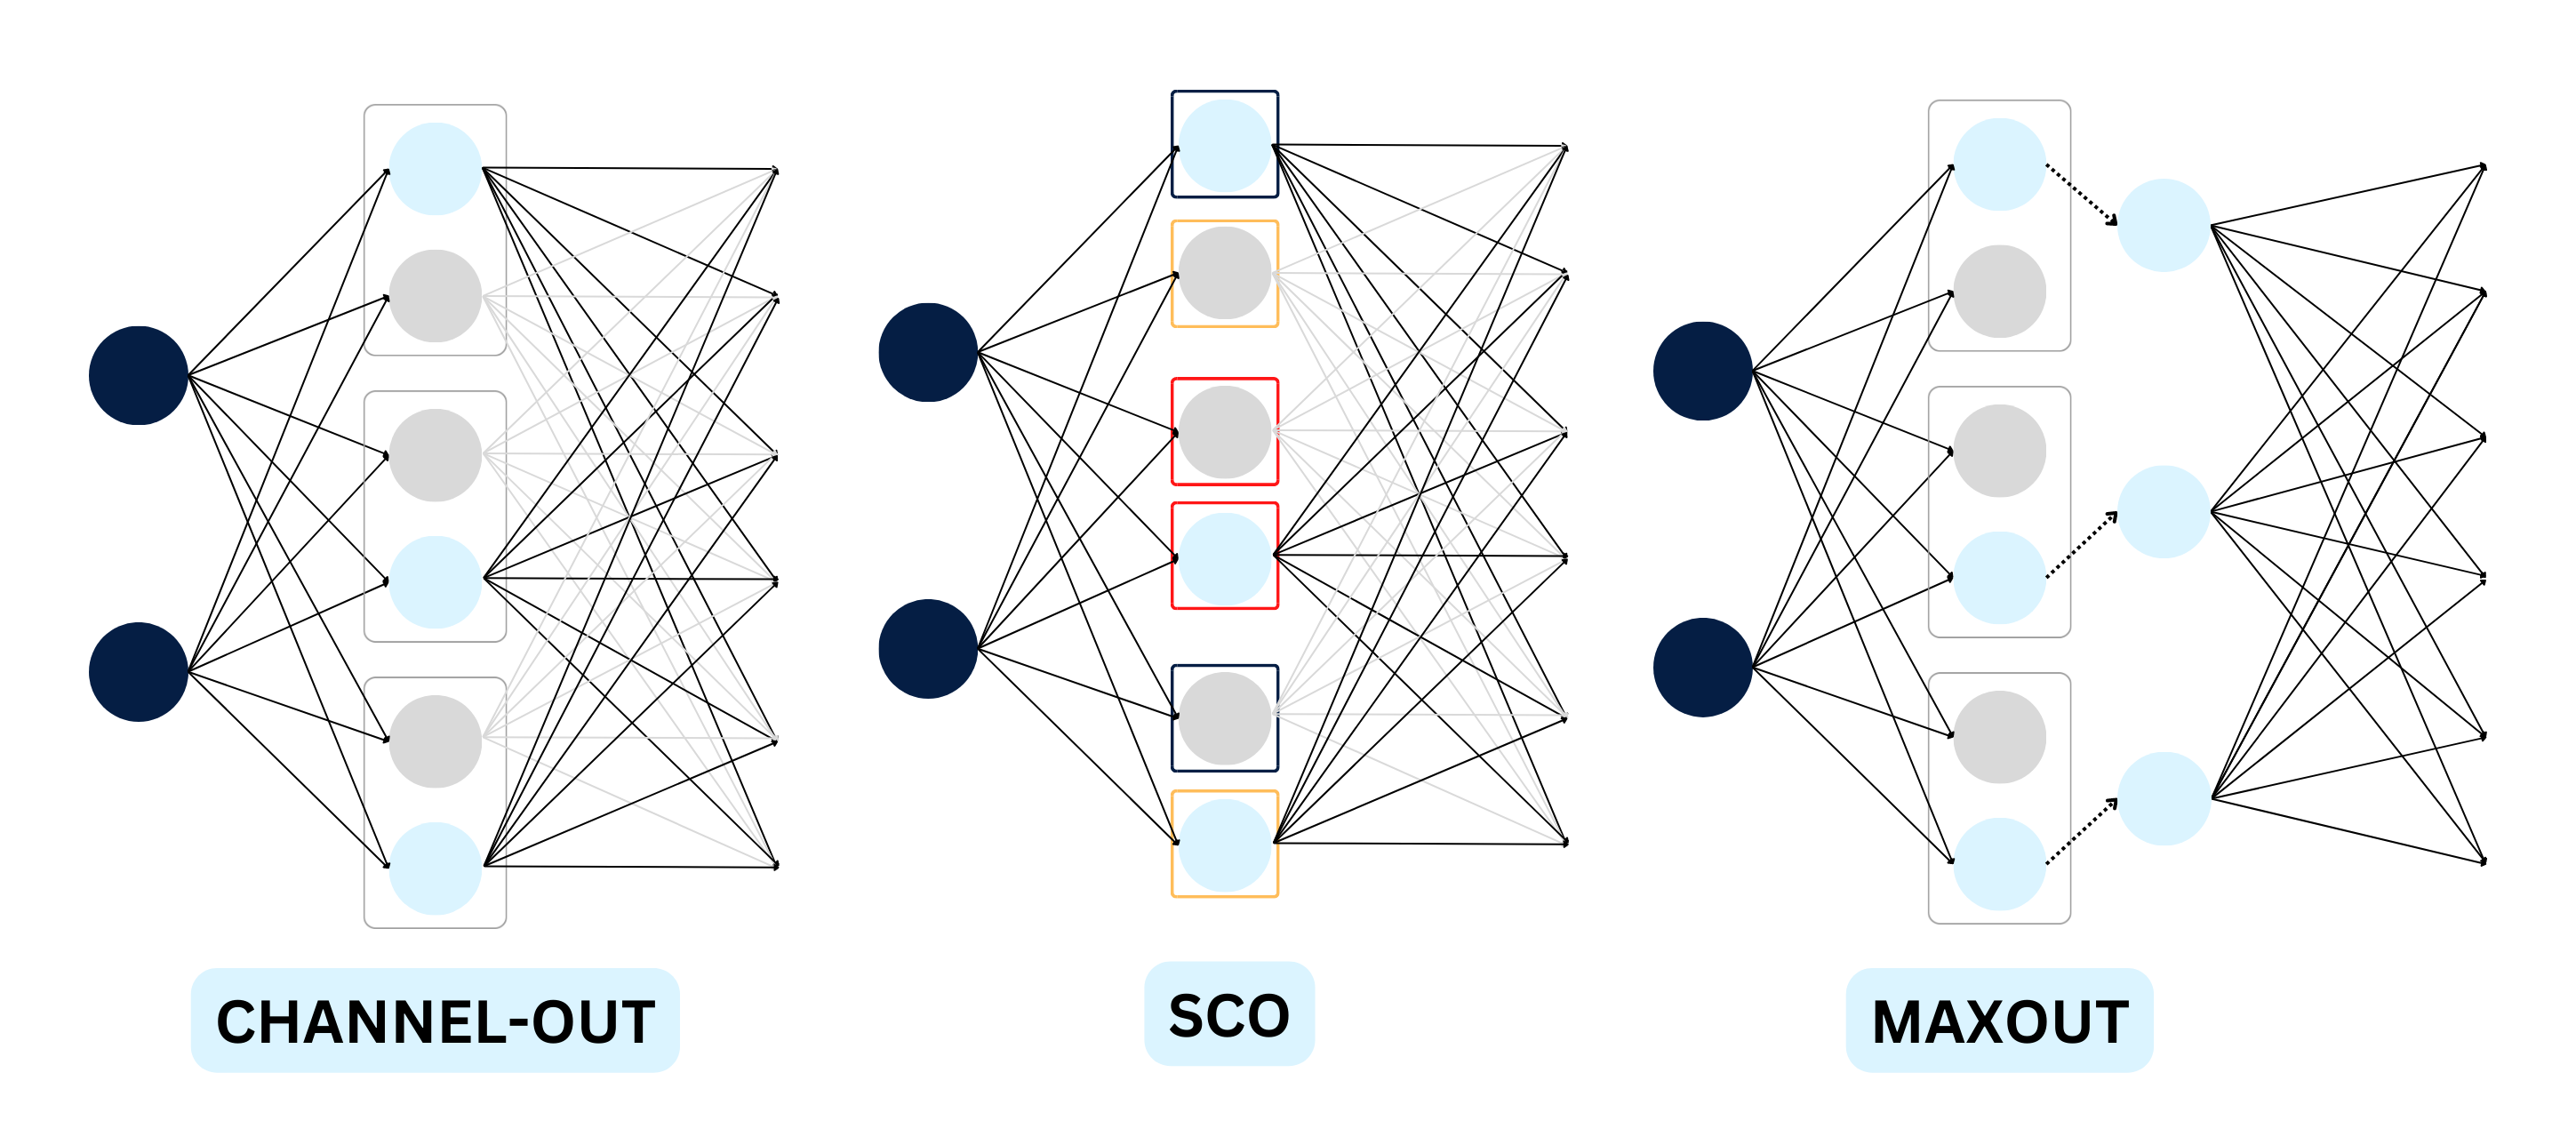
\includegraphics[width = \textwidth]{figures/EnsembleComp}
    \end{textblock}
\end{frame}

\begin{frame}{Visualization and study of sparse pathways}
    \begin{itemize}
        \item A study of the implementation \\
        and effect of LWTA layers
        \item Visualize the activation and \\
        paths of 100 randomly sampled \\
        events
        \begin{itemize}
            \item 50 background
            \item 50 signal
        \end{itemize}
        \item The bolder the line the more\\ 
        frequently the path is used.
    \end{itemize}
\end{frame}
\begin{frame}
    \begin{textblock}{0.8}(0.015, 0.25)
        \textbf{Before training}
    \end{textblock}
    \begin{textblock}{0.8}(0.017, 0.7)
        \textbf{After training}
    \end{textblock}
    \begin{center}\vspace{-0.5cm}
        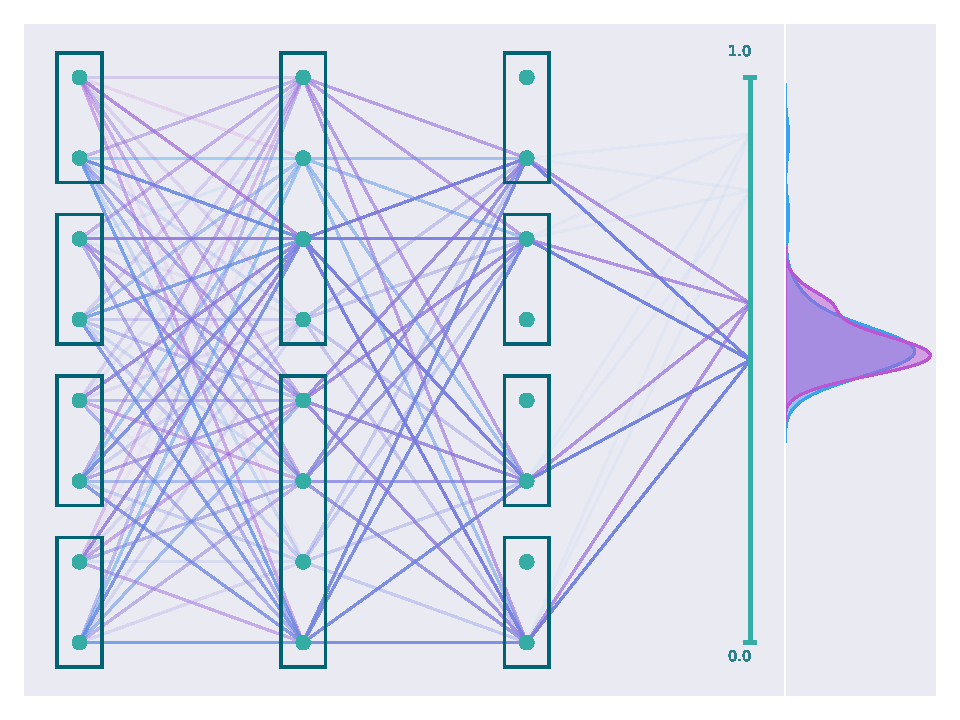
\includegraphics[width = 0.5\textwidth]{figures/NetworkVis/BeforeTraining.pdf}
        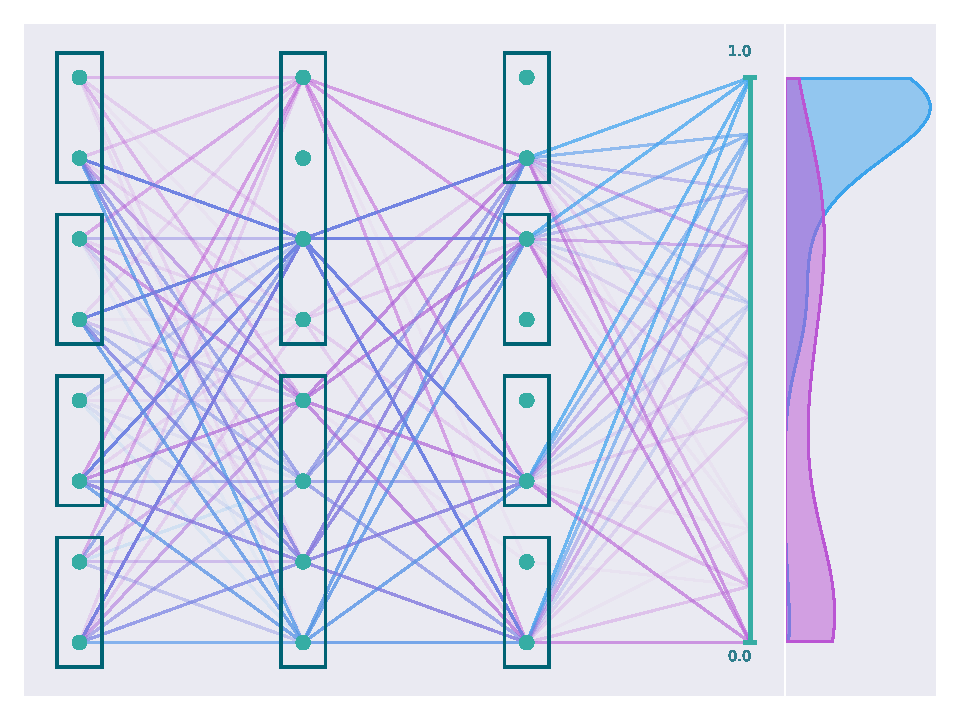
\includegraphics[width = 0.5\textwidth]{figures/NetworkVis/AfterTraining.pdf}
    \end{center}
\end{frame}
\begin{frame}
    \begin{textblock}{0.8}(0.015, 0.25)
        \textbf{Background}
    \end{textblock}
    \begin{textblock}{0.8}(0.017, 0.7)
        \textbf{Signal}
    \end{textblock}
    \begin{center}\vspace{-0.5cm}
        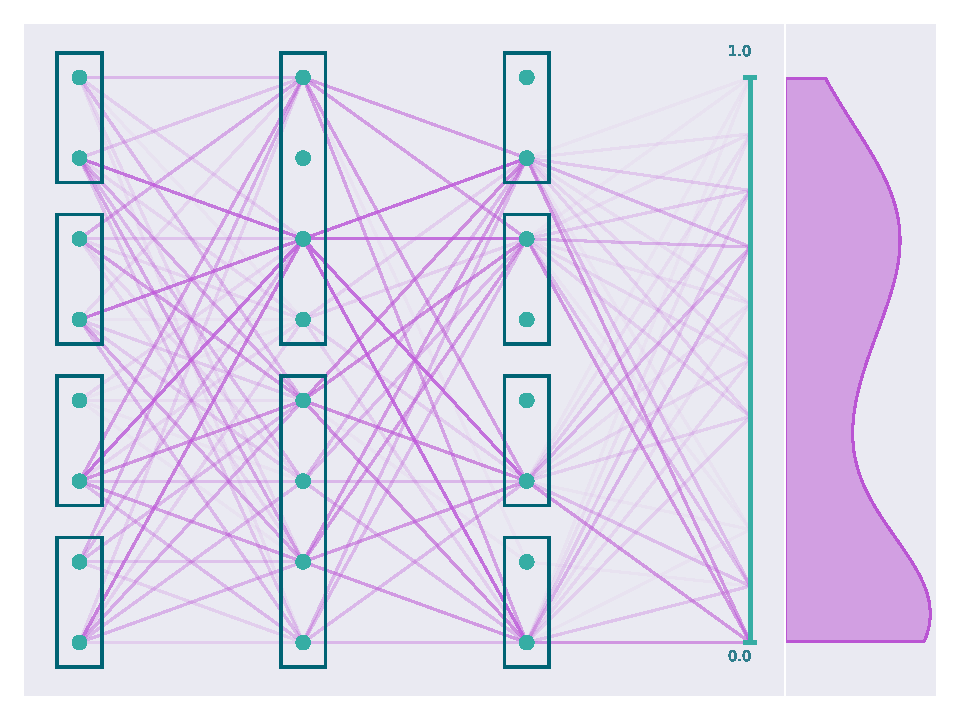
\includegraphics[width = 0.5\textwidth]{figures/NetworkVis/AfterTrainingBkg.pdf}
        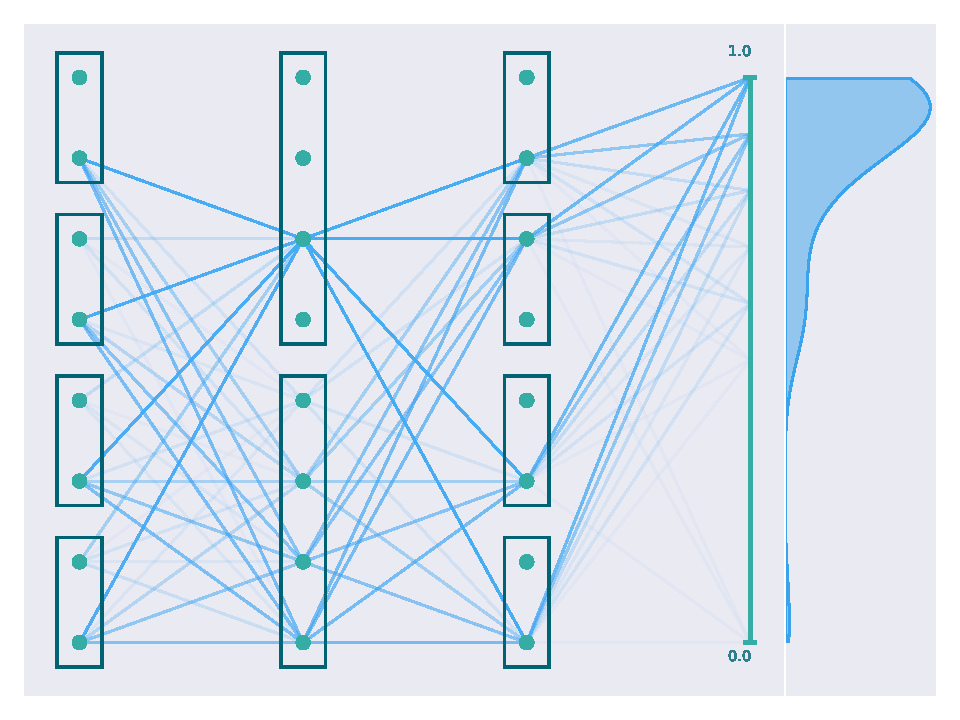
\includegraphics[width = 0.5\textwidth]{figures/NetworkVis/AfterTrainingSig.pdf}
    \end{center}
\end{frame}

\begin{frame}{Comparing activation of Maxout with SCO}
    \begin{textblock}{0.8}(0.225, 0.8)
        \textbf{Maxout}
    \end{textblock}
    \begin{textblock}{0.8}(0.7, 0.8)
        \textbf{SCO}
    \end{textblock}
    \vfill
    \begin{center}
        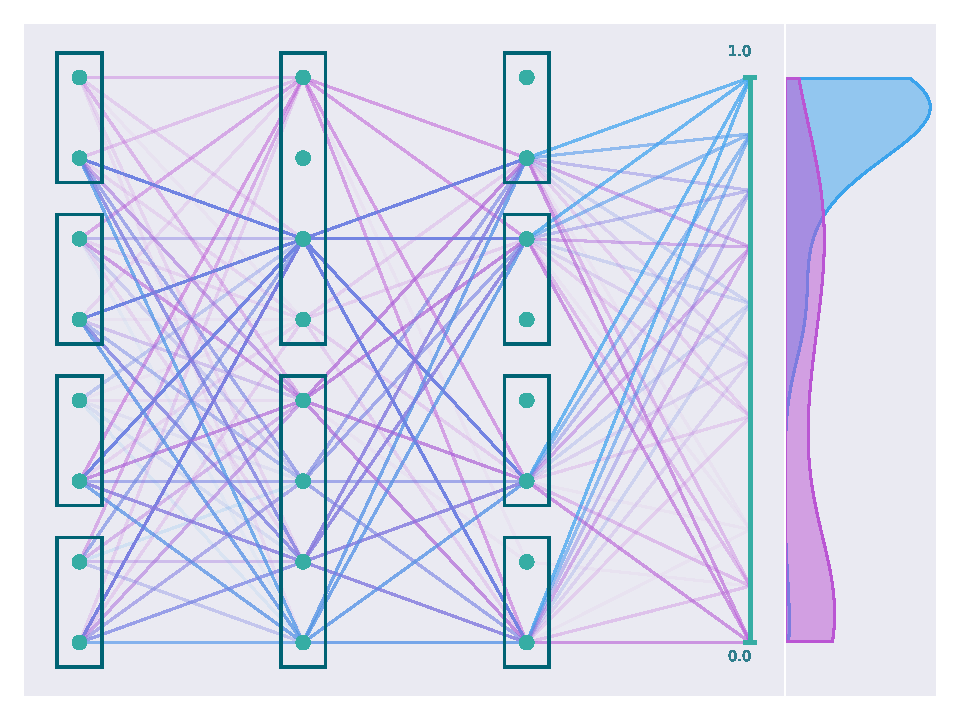
\includegraphics[width = 0.475\textwidth]{figures/NetworkVis/AfterTraining.pdf}
        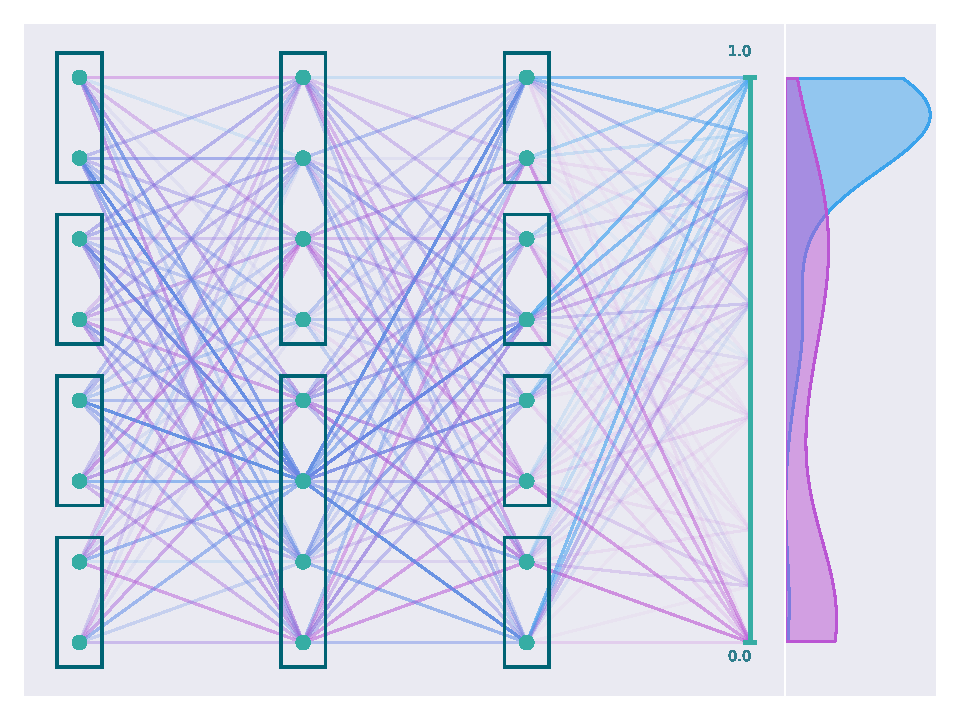
\includegraphics[width = 0.475\textwidth]{figures/NetworkVis/SCO/AfterTraining.pdf}
    \end{center}
\end{frame}
\begin{frame}{Ensemble network architecture}
    \vfill
    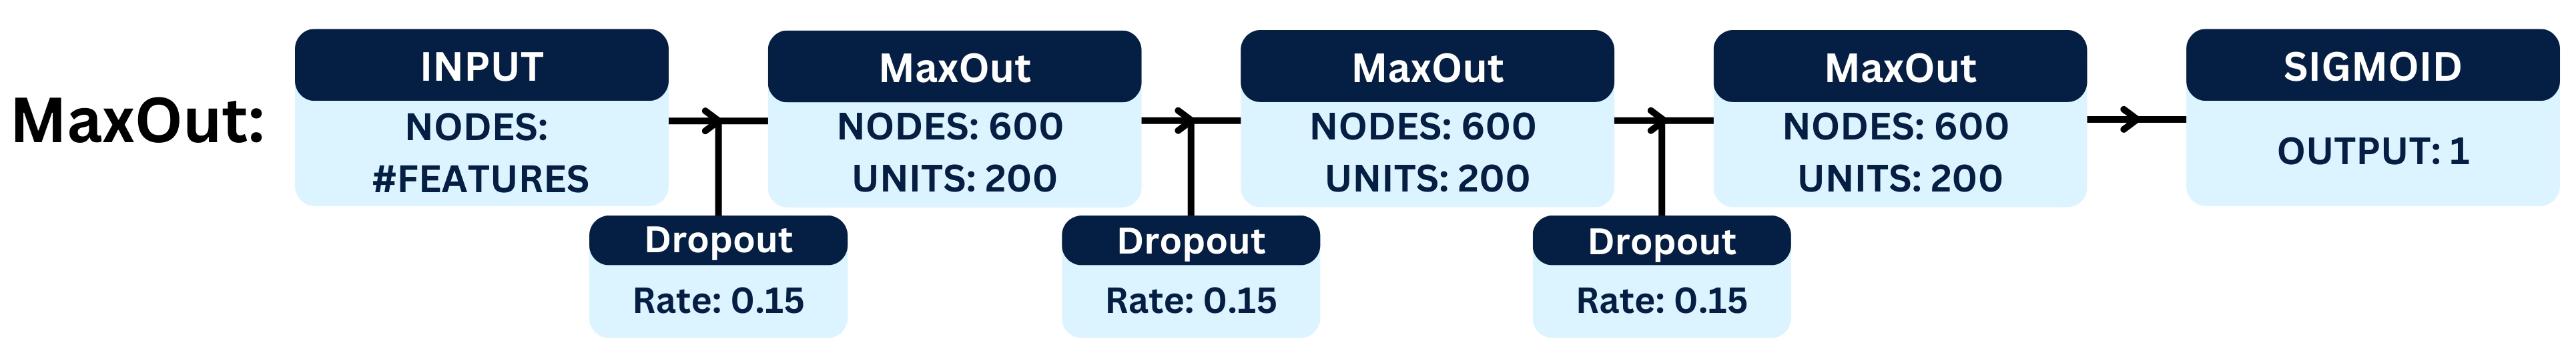
\includegraphics[width = 0.98\textwidth]{figures/maxout.png}
\end{frame}
\begin{frame}{Comparing sensitivity of channel-out, SCO and maxout}
    \begin{textblock}{1}(-0.0375, 0.2)
        \begin{itemize}
            \item Maxout: 23/30
            \item SCO: 7/30
            \begin{itemize}
                \item No trend for \\
                preferred masses
                \item Possibly improve\\
                      without layer on \\
                      prediction 
            \end{itemize}
        \end{itemize}
    \end{textblock}
    \begin{textblock}{1}(0.33, 0.2)
    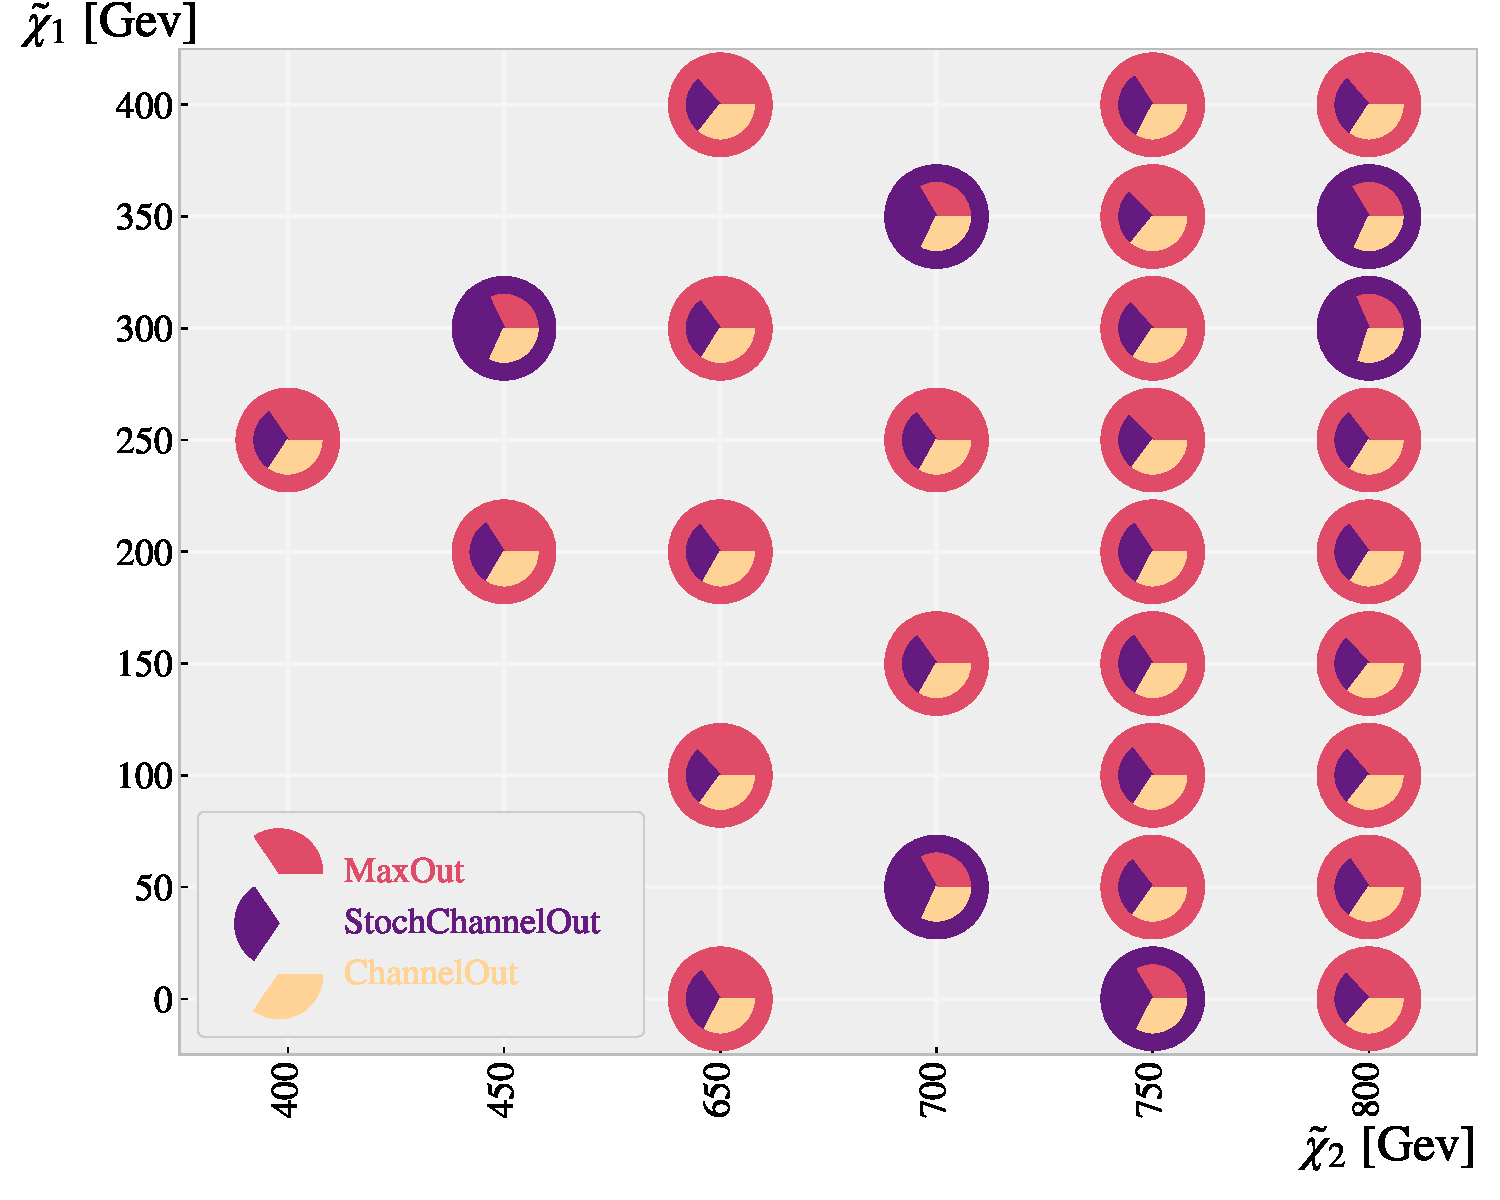
\includegraphics[width = 0.625\textwidth]{figures/Comps/EnsemblesNetworkComp.pdf}
    \end{textblock}
\end{frame}
% \begin{frame}
%     \begin{center}
%         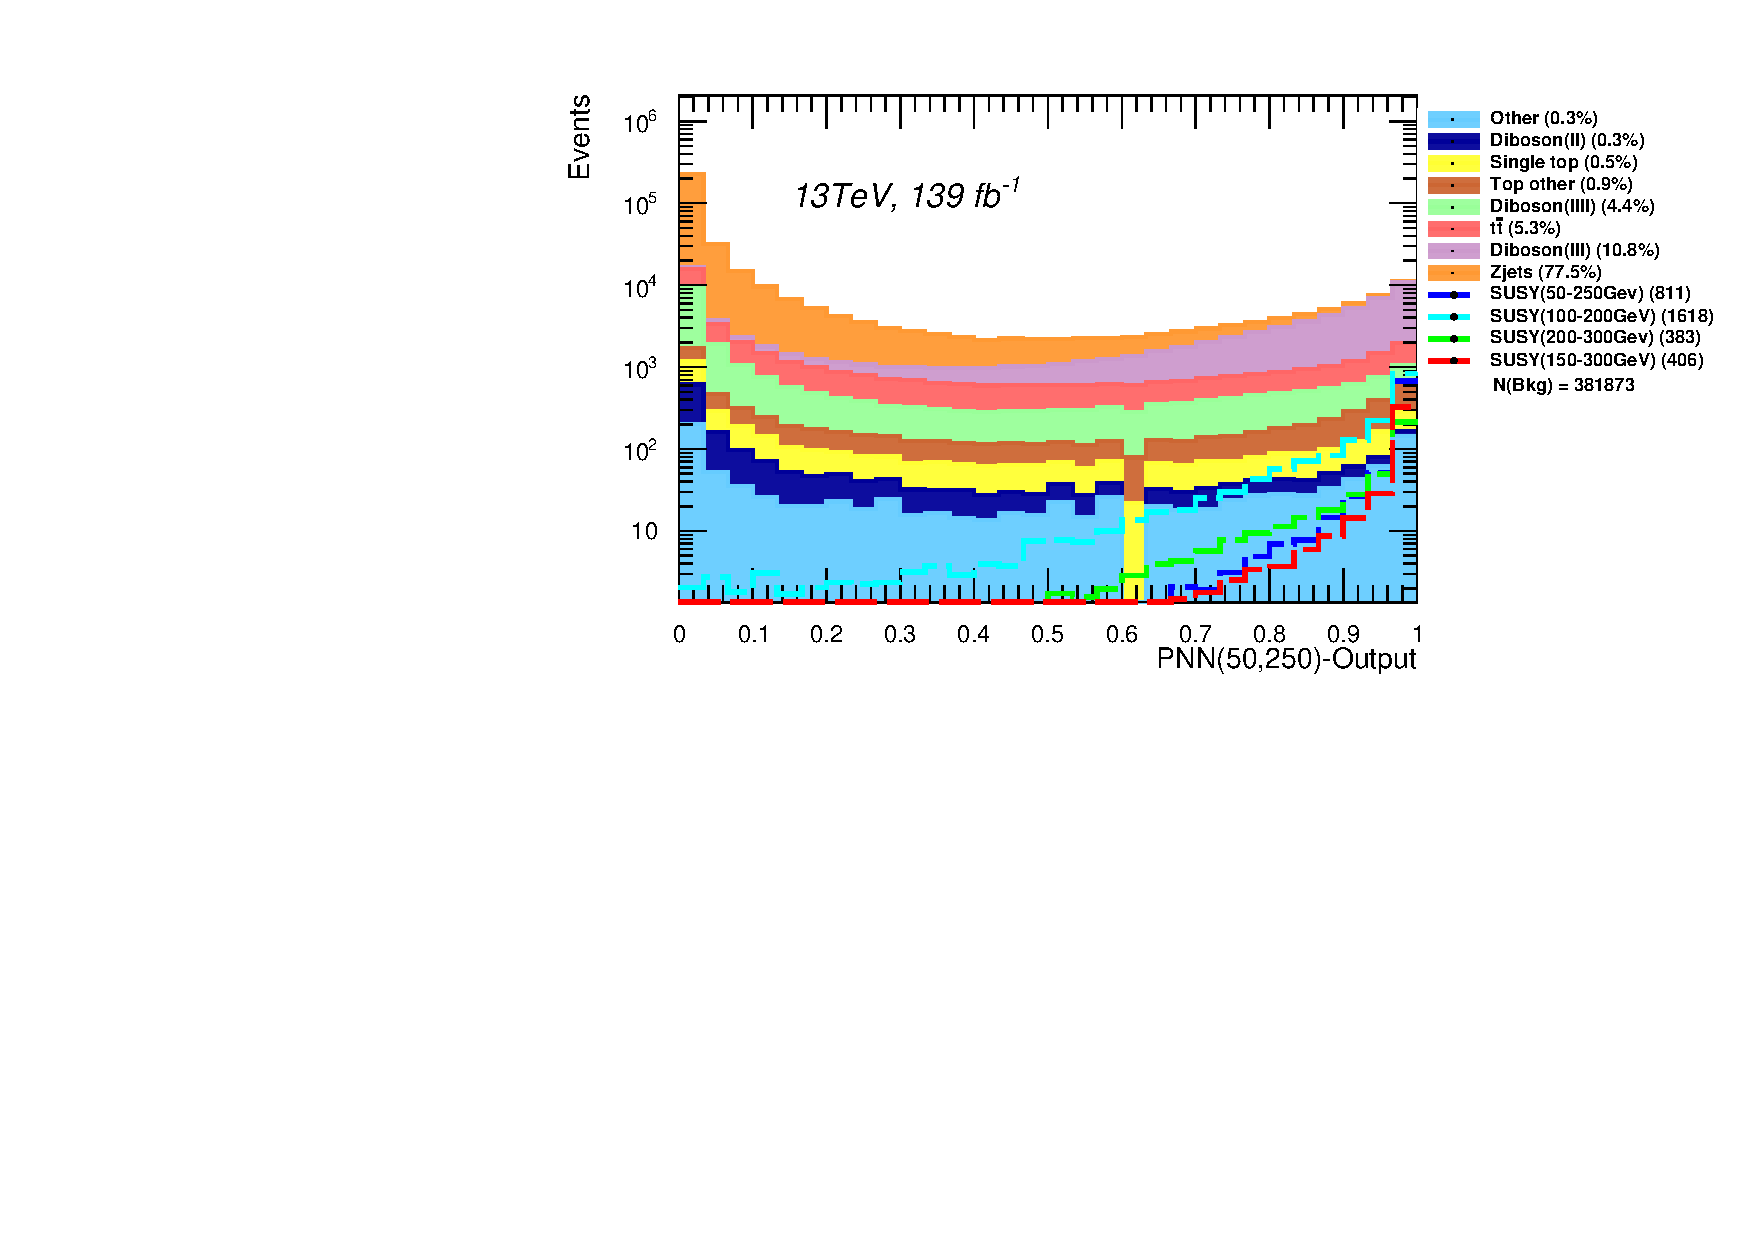
\includegraphics[width = 0.475\textwidth]{figures/PNN/PNN50250Dist.pdf}
%         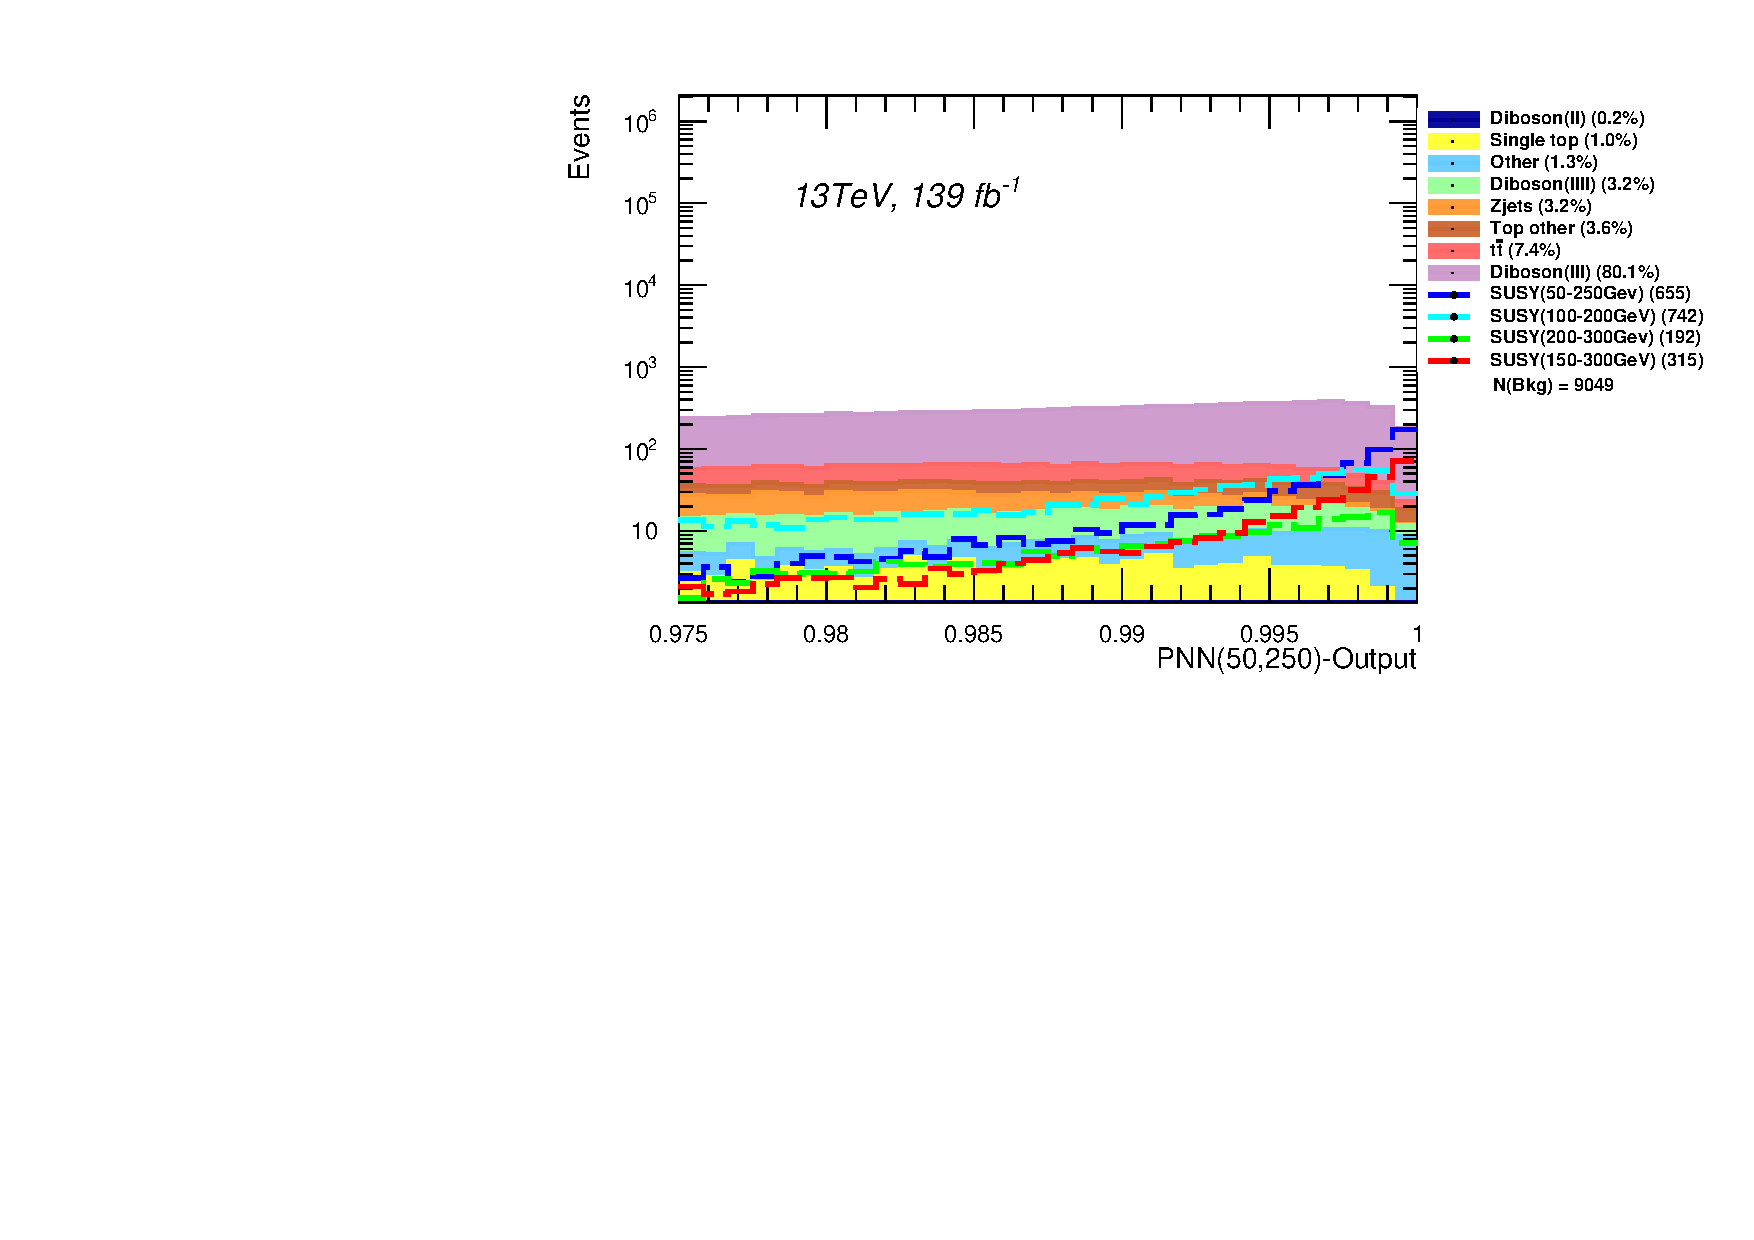
\includegraphics[width = 0.475\textwidth]{figures/PNN/PNN50250Dist_C7.pdf}
%     \end{center}
%     \begin{center}
%         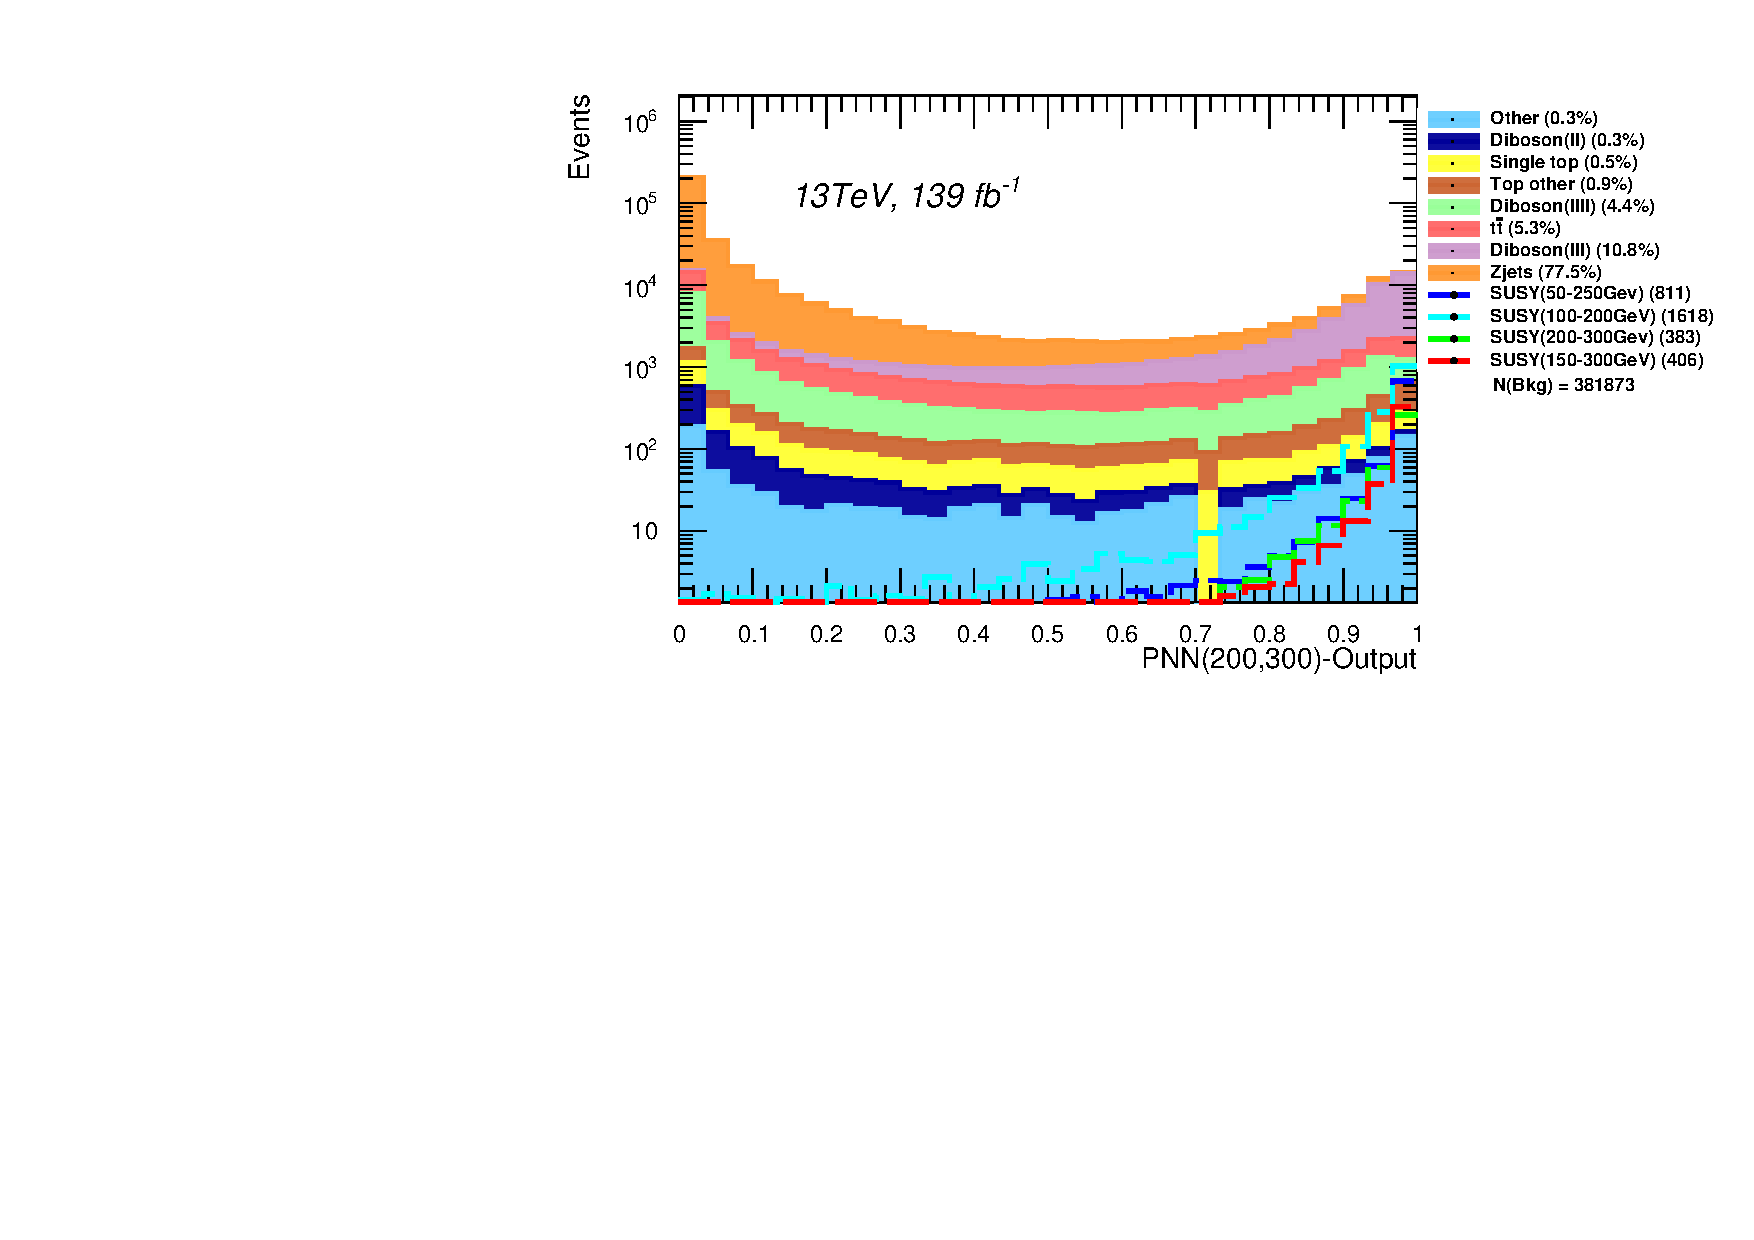
\includegraphics[width = 0.475\textwidth]{figures/PNN/PNN200300Dist.pdf}
%         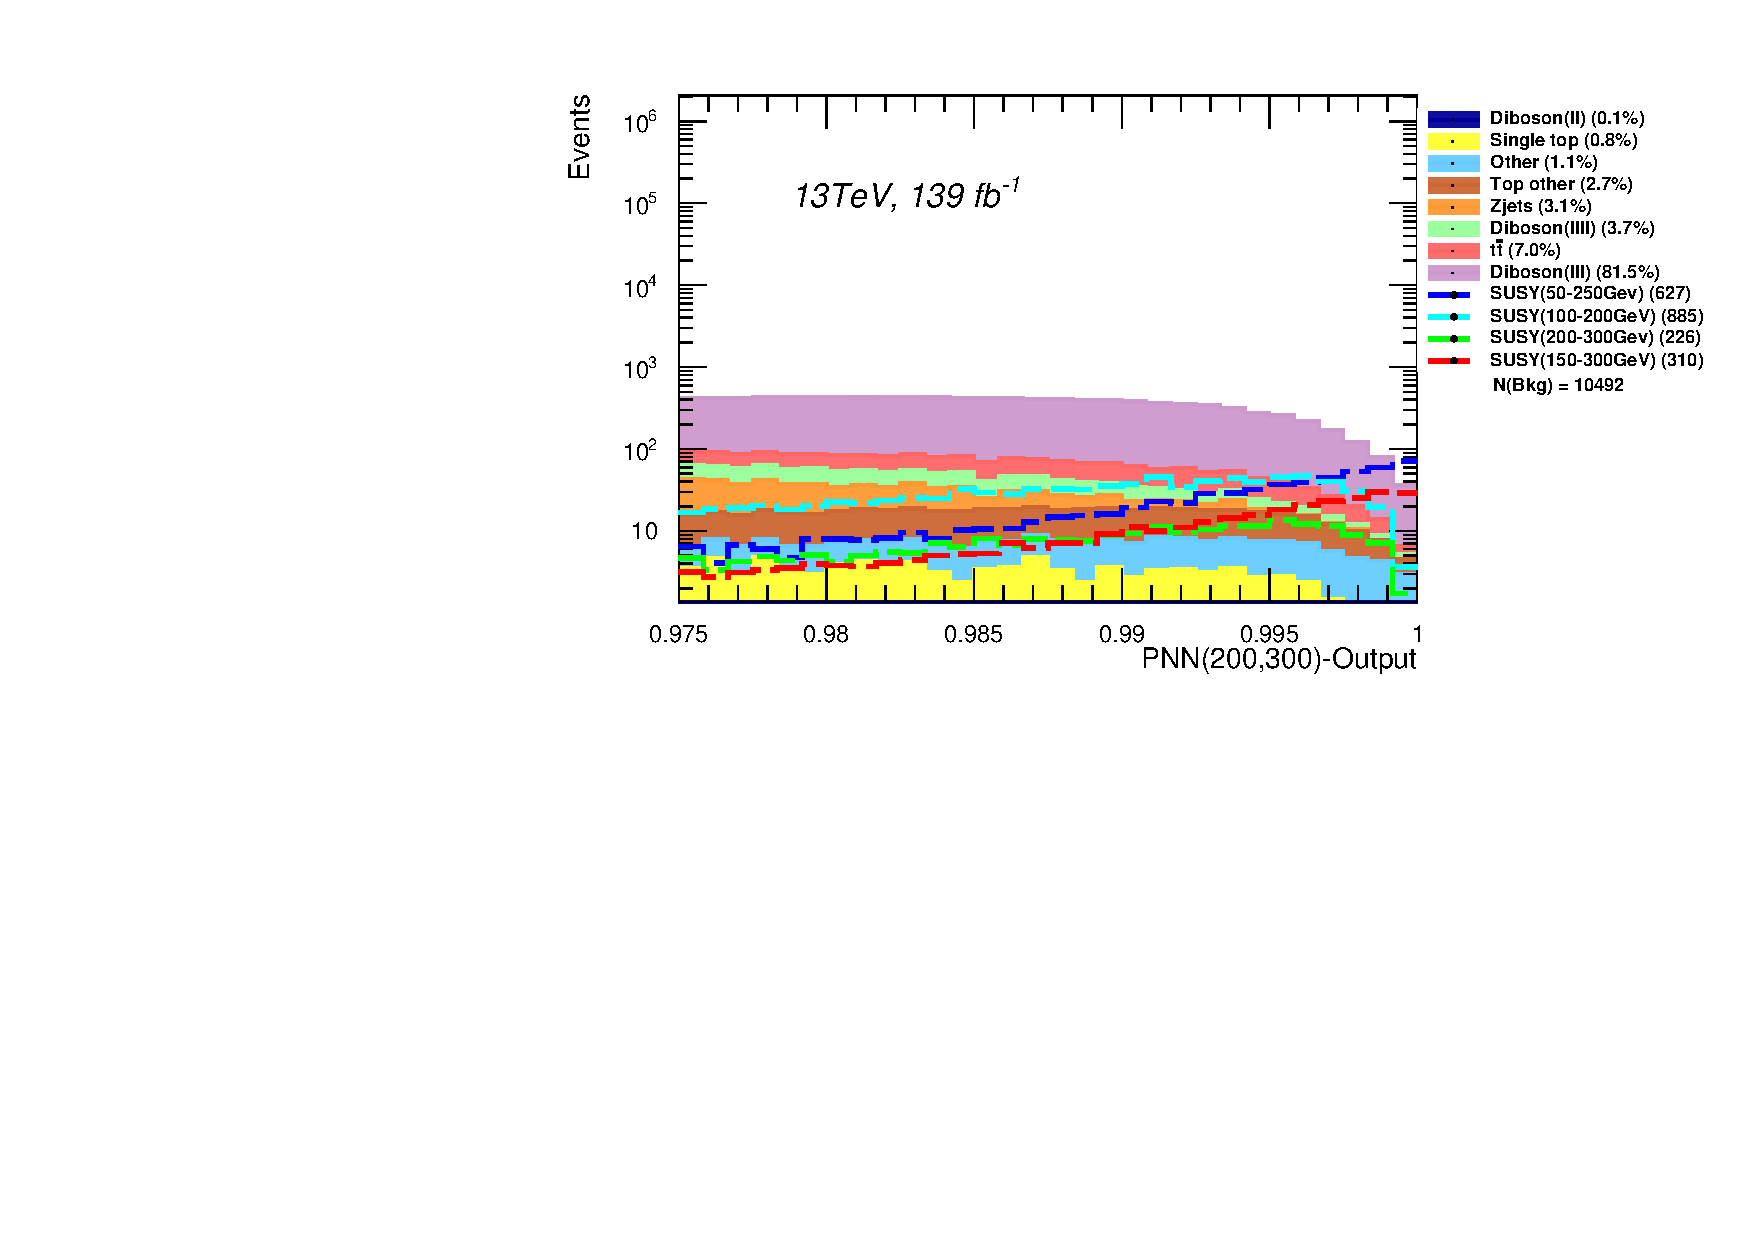
\includegraphics[width = 0.475\textwidth]{figures/PNN/PNN200300Dist_C7.pdf}
%     \end{center}
% \end{frame}

% \begin{frame}{Efficiency table}
%     \vfill
%     \begin{table}
%         \scriptsize
%         \centering
%         $
%         \begin{array}{cccccc}
%             \hline \text { \diagbox{\textbf{Parameters}}{\textbf{Channel}} }  & \text {$(50,250)$} & \text {$(100,200)$} & \text {$(150,300)$} & \text {$(200,300)$} & \text {$(Background)$} \\
%             \hline \text {$(50,250)$}   & \text { $\bf{80.8}\%$ } & \text { $45.8\%$ } & \text { $\bf{77.5}\%$ } & \text { $50.1\%$ } & \text { $2.4\%$ }  \\
%             \text {$(200,300)$}   & \text { $77.3\%$ } & \text { $\bf{54.6}\%$ } & \text { $76.3\%$ } & \text { $\bf{59.0}\%$ } & \text { $2.74\%$ }\\
%             \hline
%         \end{array}
%         $
%     \end{table}
% \end{frame}

\begin{frame}{Comparing the sensitivity on a subset of the signal}
    \centering
    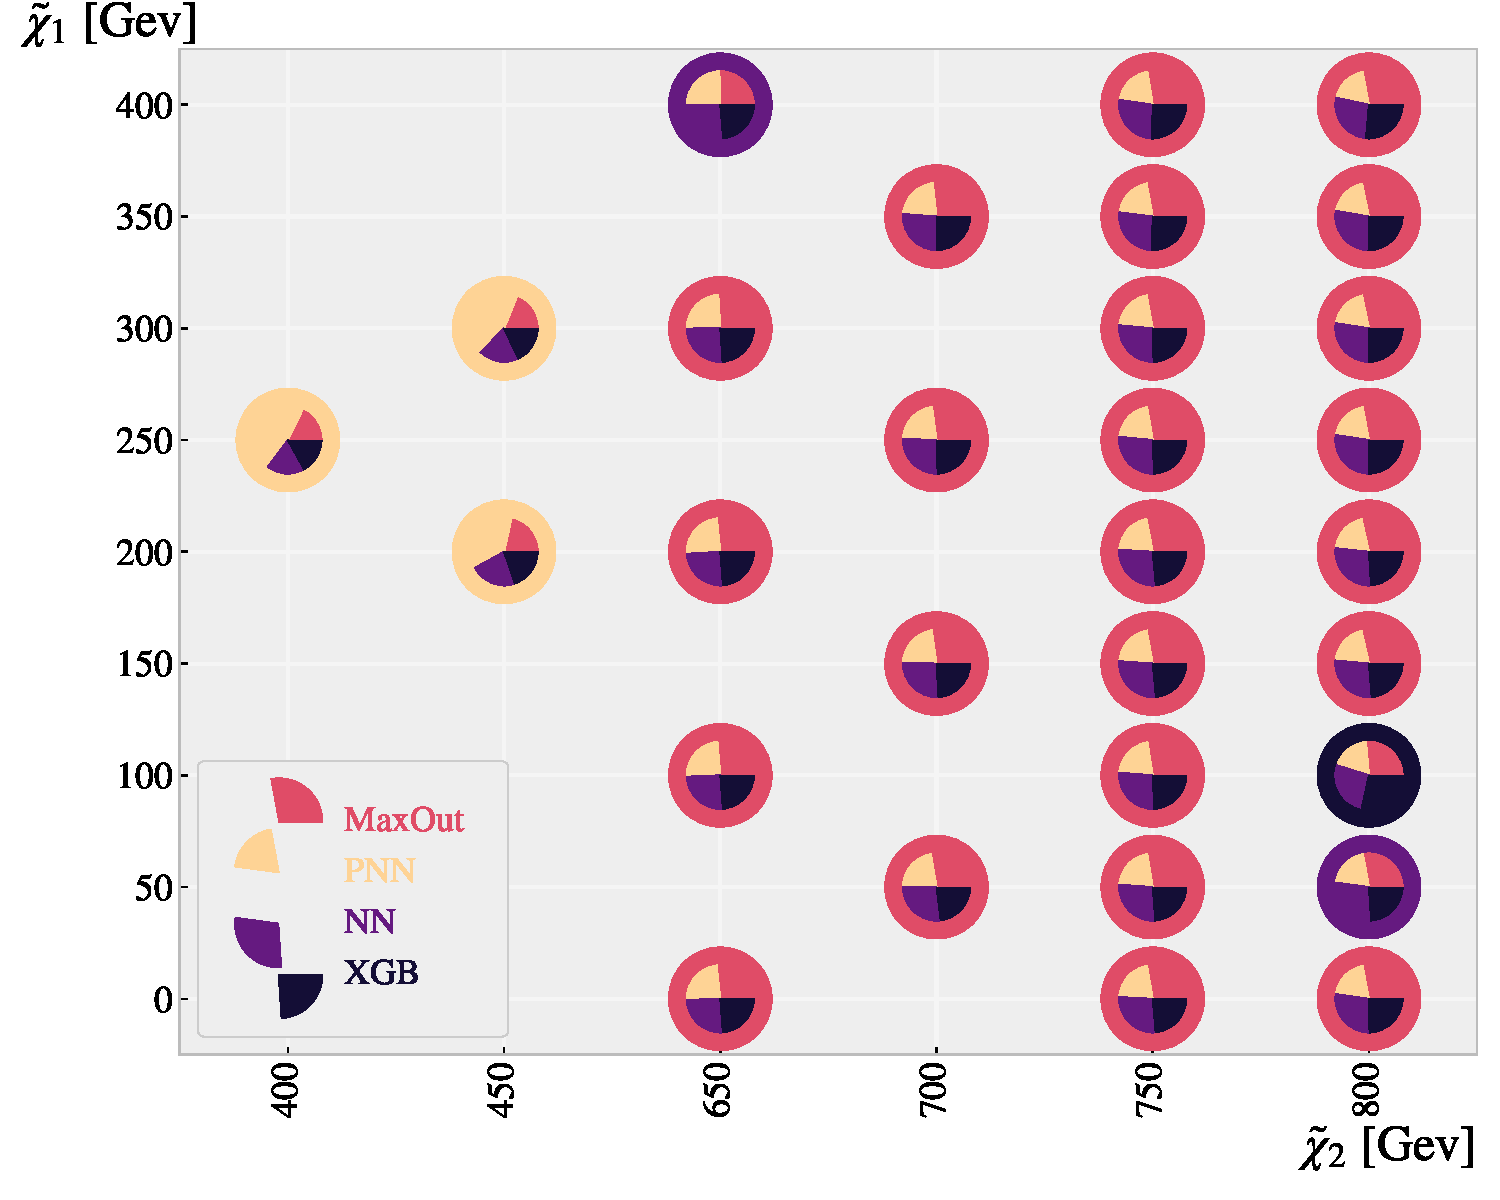
\includegraphics[width=0.75\textwidth]{figures/Comps/GenPlussXGBNetworkComp.pdf}
\end{frame}


\begin{frame}{Increasing sensitivity through a PCA}
        \begin{itemize}
            \item Dimensionality reduction
            \item Creates new features using linear combination of original features
            \item Ranks from most to least variance
            \item This analysis
            \begin{itemize}
                \item Demand conservation of $99.9\%$ of variance/spread
                \item 5 features removed
            \end{itemize}
        \end{itemize}
\end{frame}
\begin{frame}{Compare methods with and without PCA}
    \begin{textblock}{0.8}(0.02, 0.3)
        {Maxout}
    \end{textblock}
    \begin{textblock}{0.8}(0.9, 0.3)
        {PNN}
    \end{textblock}
    \begin{textblock}{0.8}(0.275, 0.7)
    {NN}
    \end{textblock}
    \begin{center}
        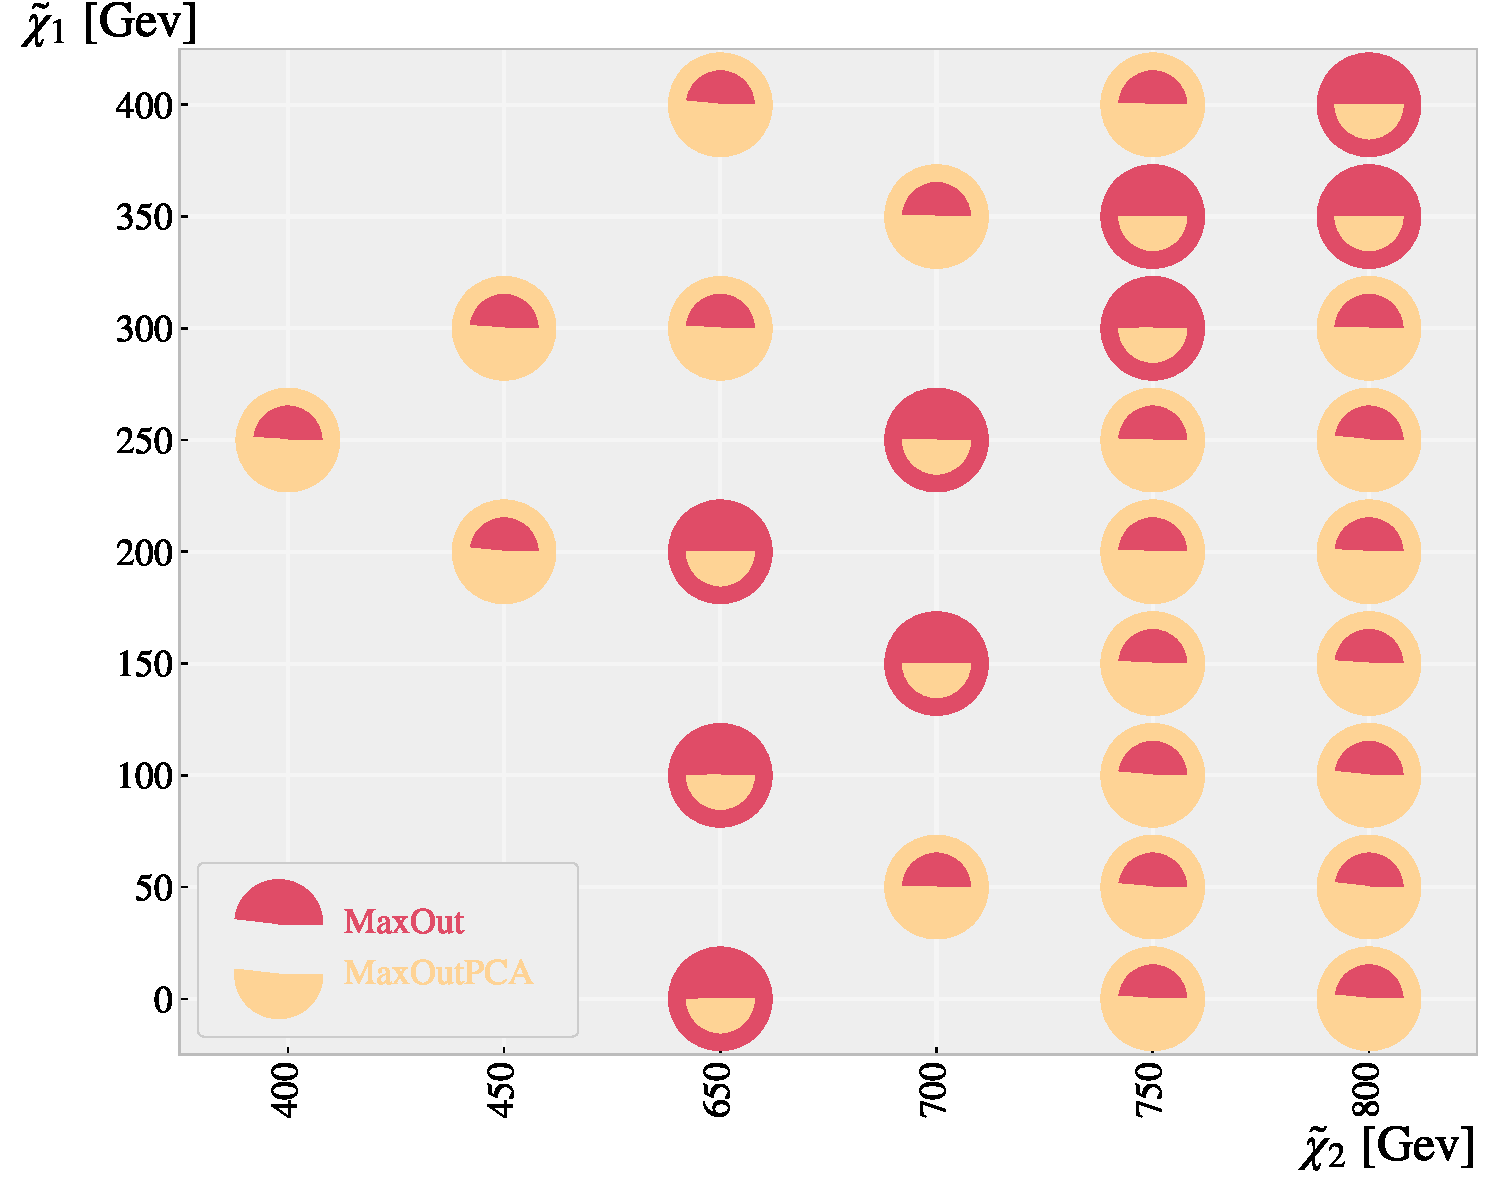
\includegraphics[width=0.415\textwidth]{figures/Comps/MaxOutPCANetworkComp.pdf}
        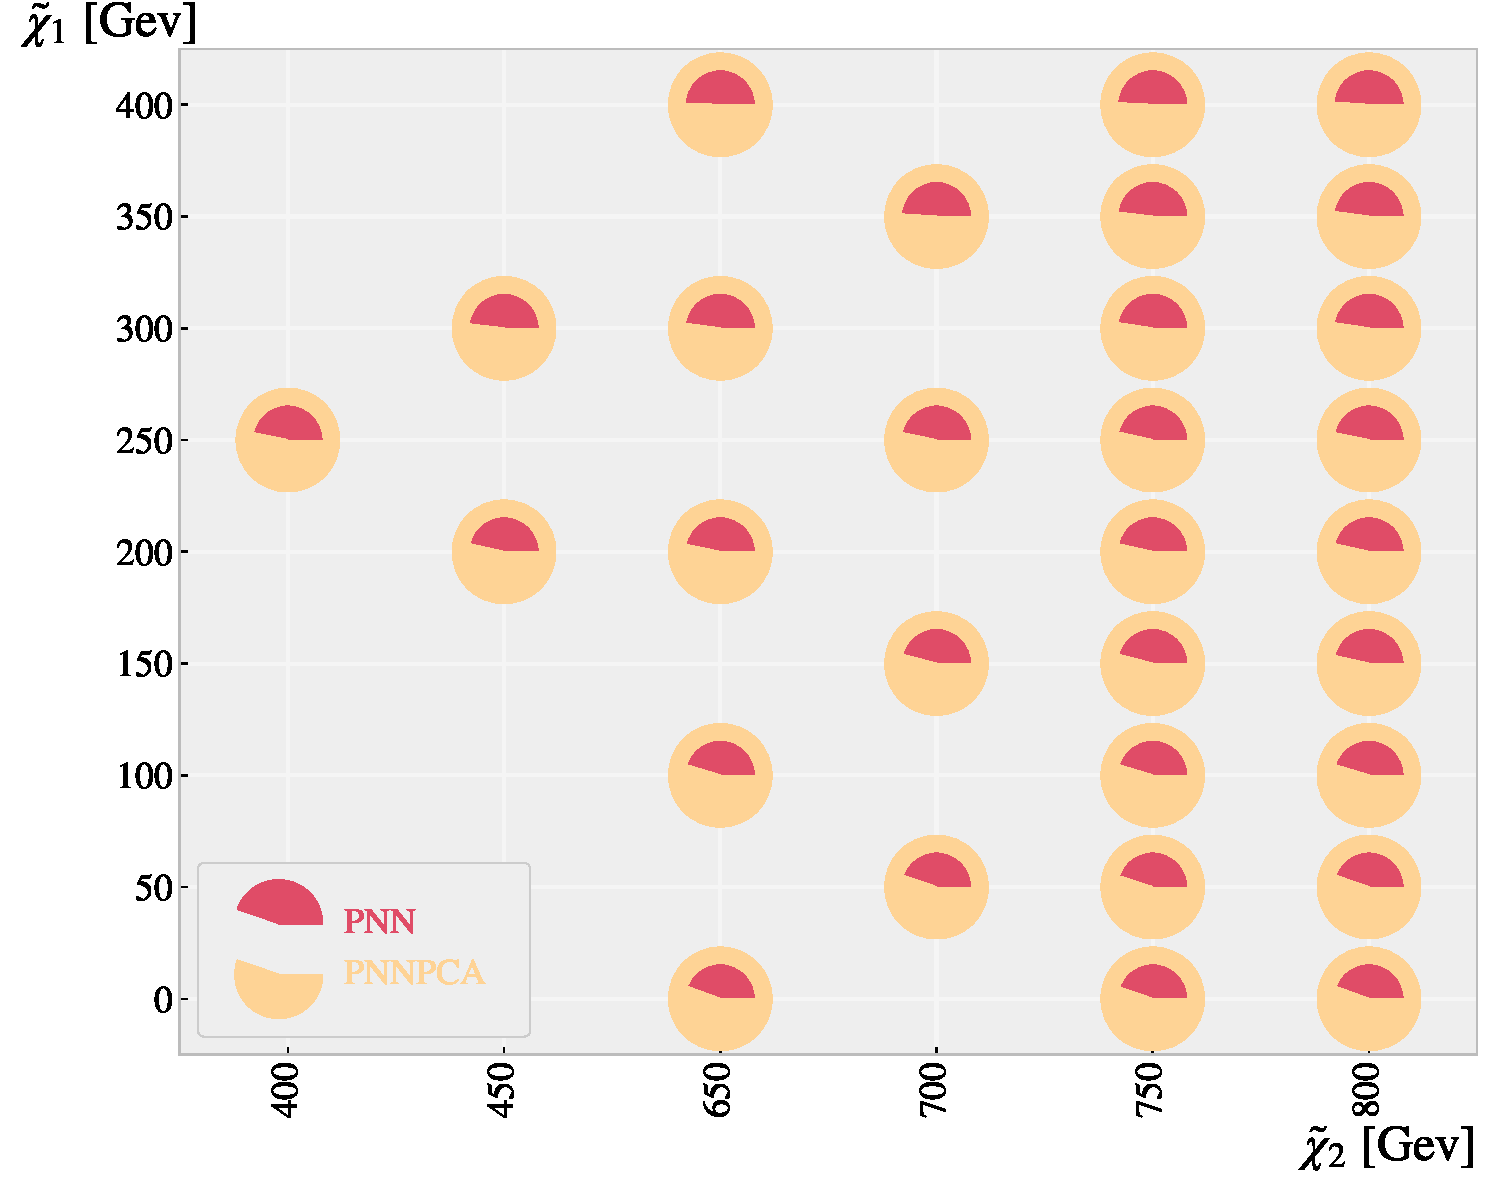
\includegraphics[width=0.415\textwidth]{figures/Comps/PNNPCANetworkComp.pdf}
    \end{center}
    \centering
    \vspace{-0.2cm}
    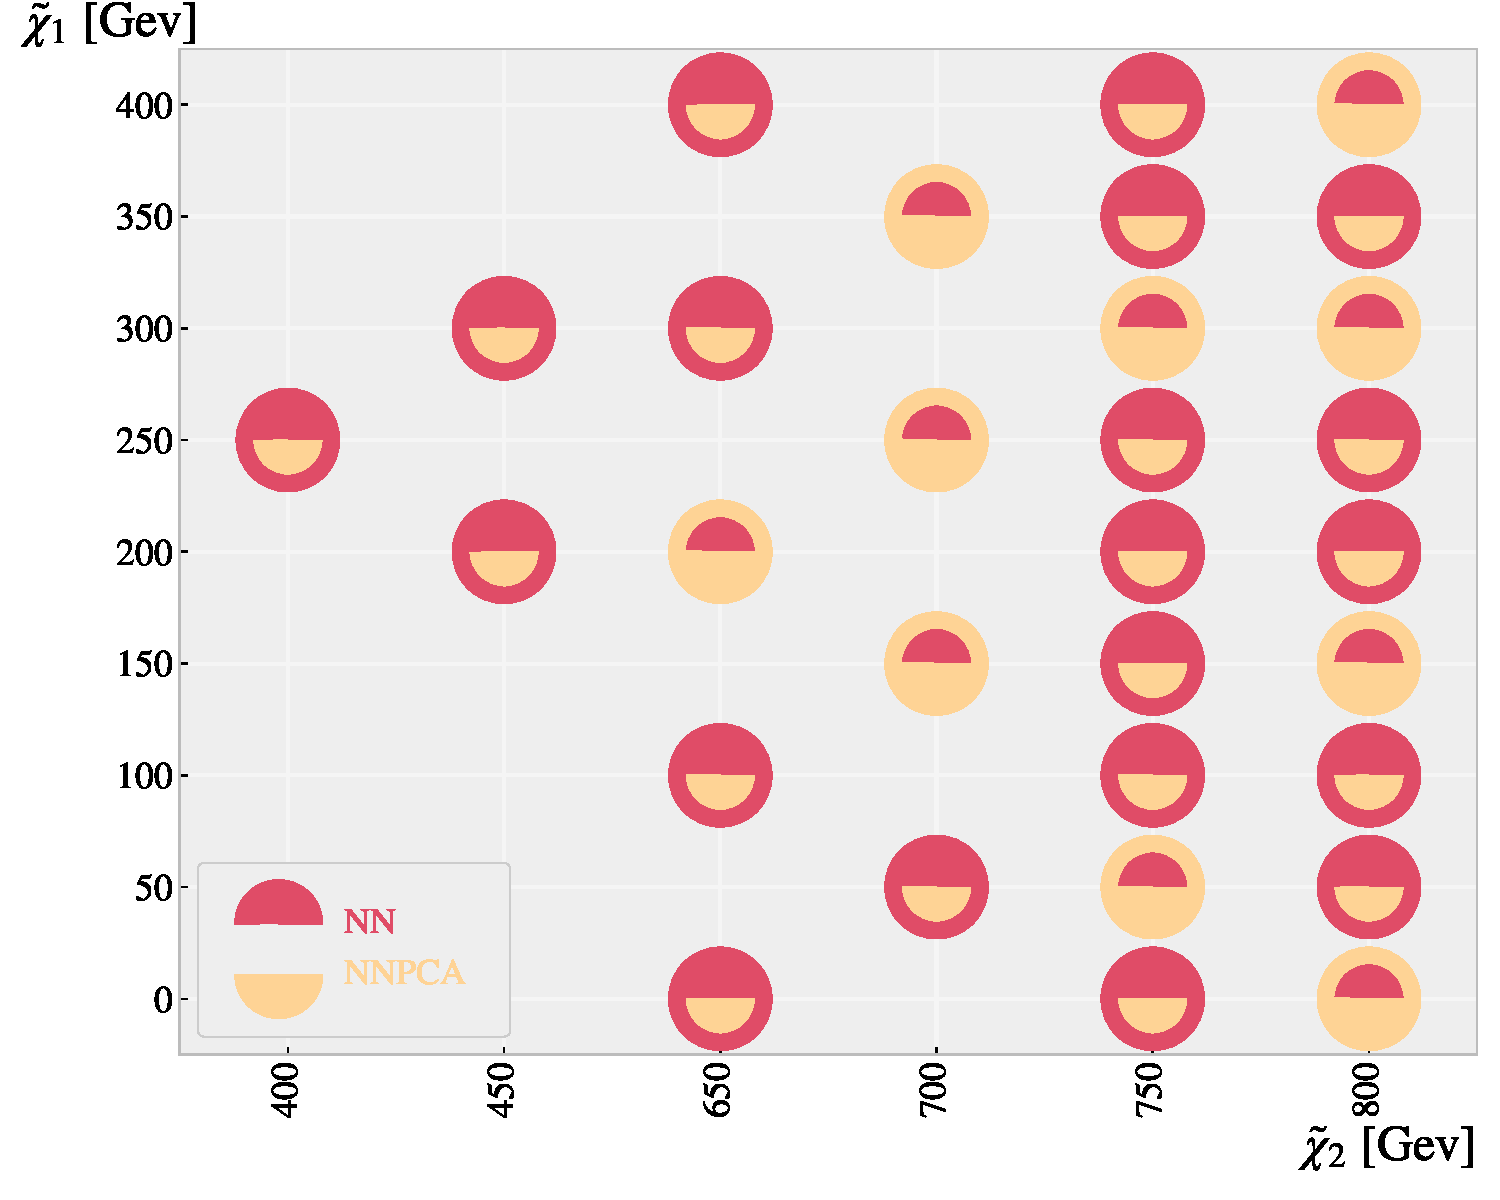
\includegraphics[width=0.415\textwidth]{figures/Comps/NNPCANetworkComp.pdf}

\end{frame}


\begin{frame}{Comparing the methods to previous analysis}
    \begin{itemize}
        \item Compare the expected limits of three best models
              to analysis made by ATLAS in 2021 \cite{atlas_search_2021}
        \item Introduce flat uncertainty for realistic comparison ($20\%$, $10\%$, $<1\%$) 
        \item Include top performing methods
        \begin{itemize}
            \item Maxout model with PCA
            \item PNN with PCA
            \item Ordinary dense neural network without PCA
        \end{itemize}
    \end{itemize}
\end{frame}
\begin{frame}
    \centering
    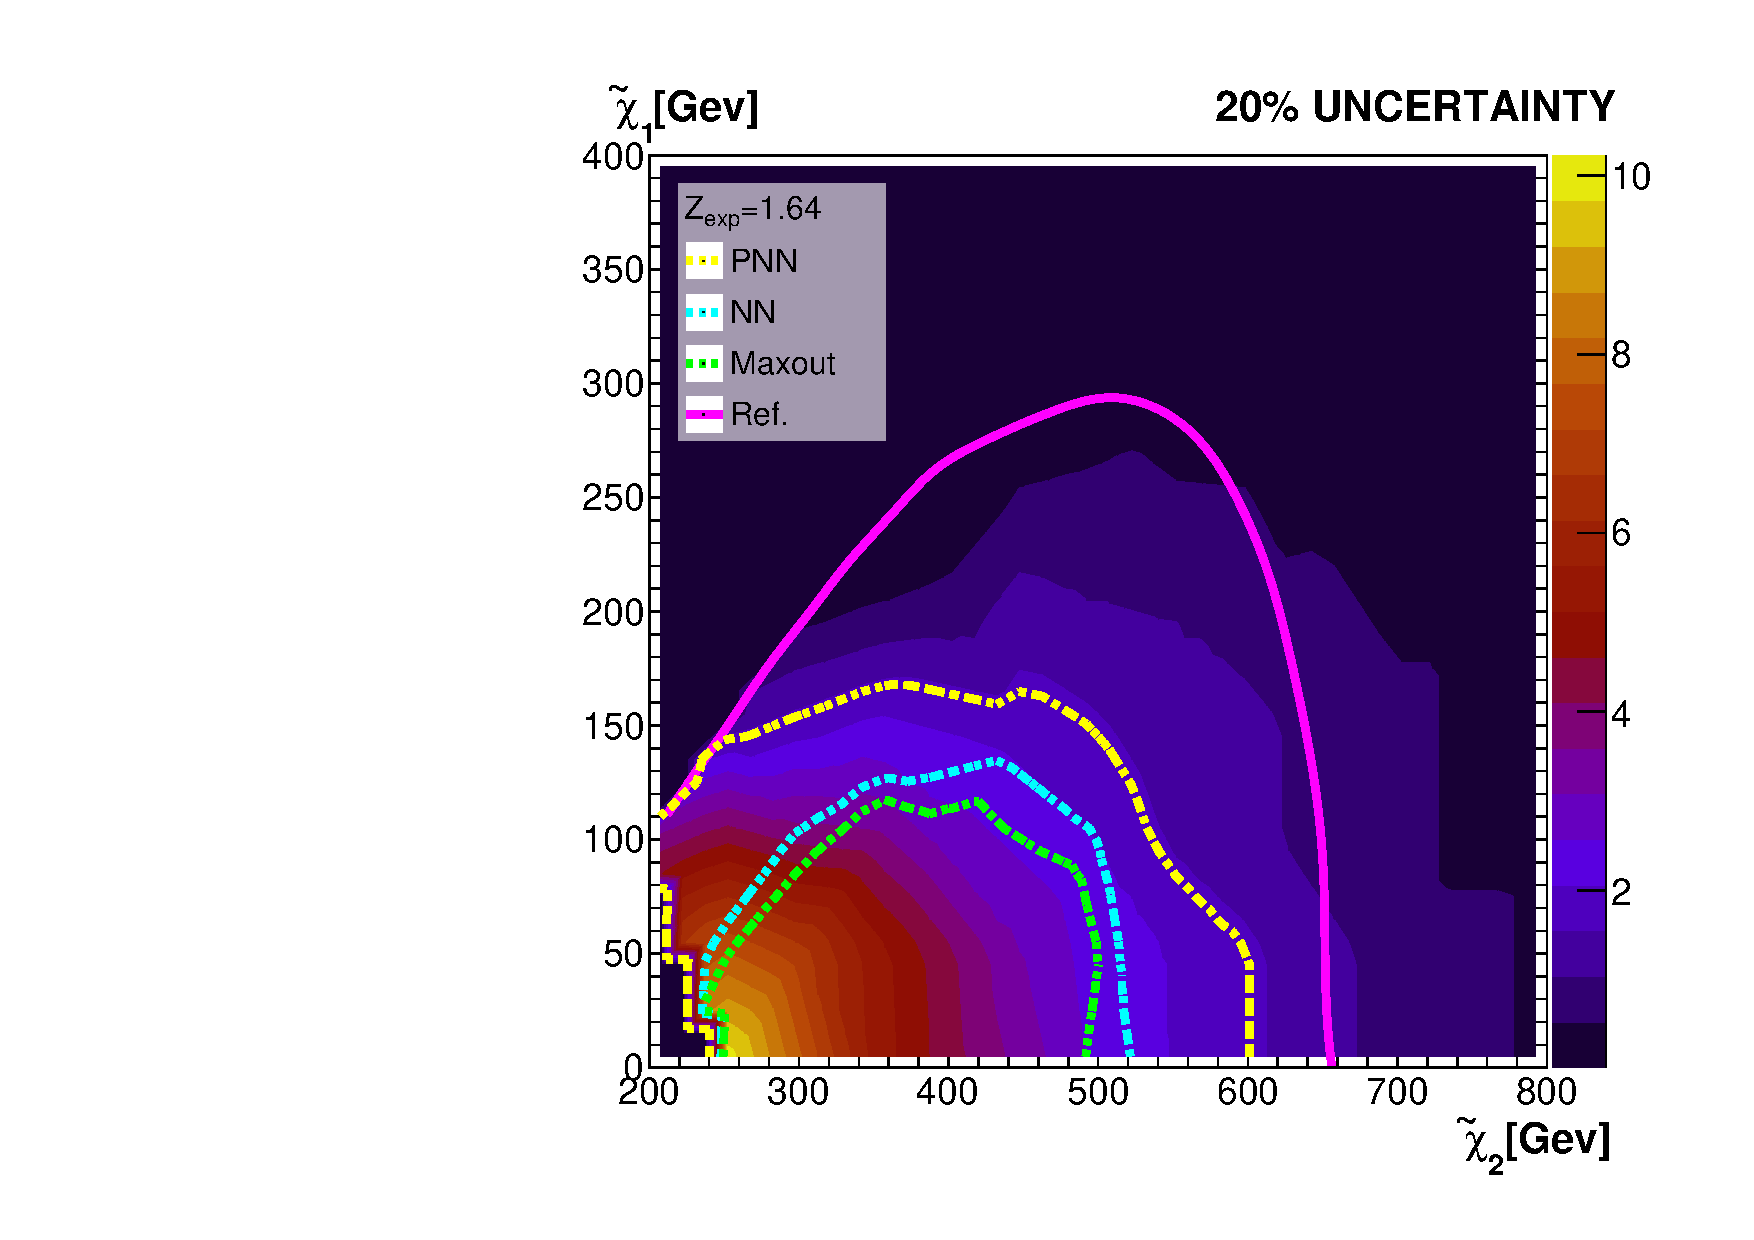
\includegraphics[width=0.7\textwidth]{figures/Limits/compLimit20.pdf}
    \begin{textblock}{1}(-0.168,.305)
        \scriptsize
        \cite{atlas_search_2021}
    \end{textblock}
\end{frame}
\begin{frame}
    \vfill
    \centering
    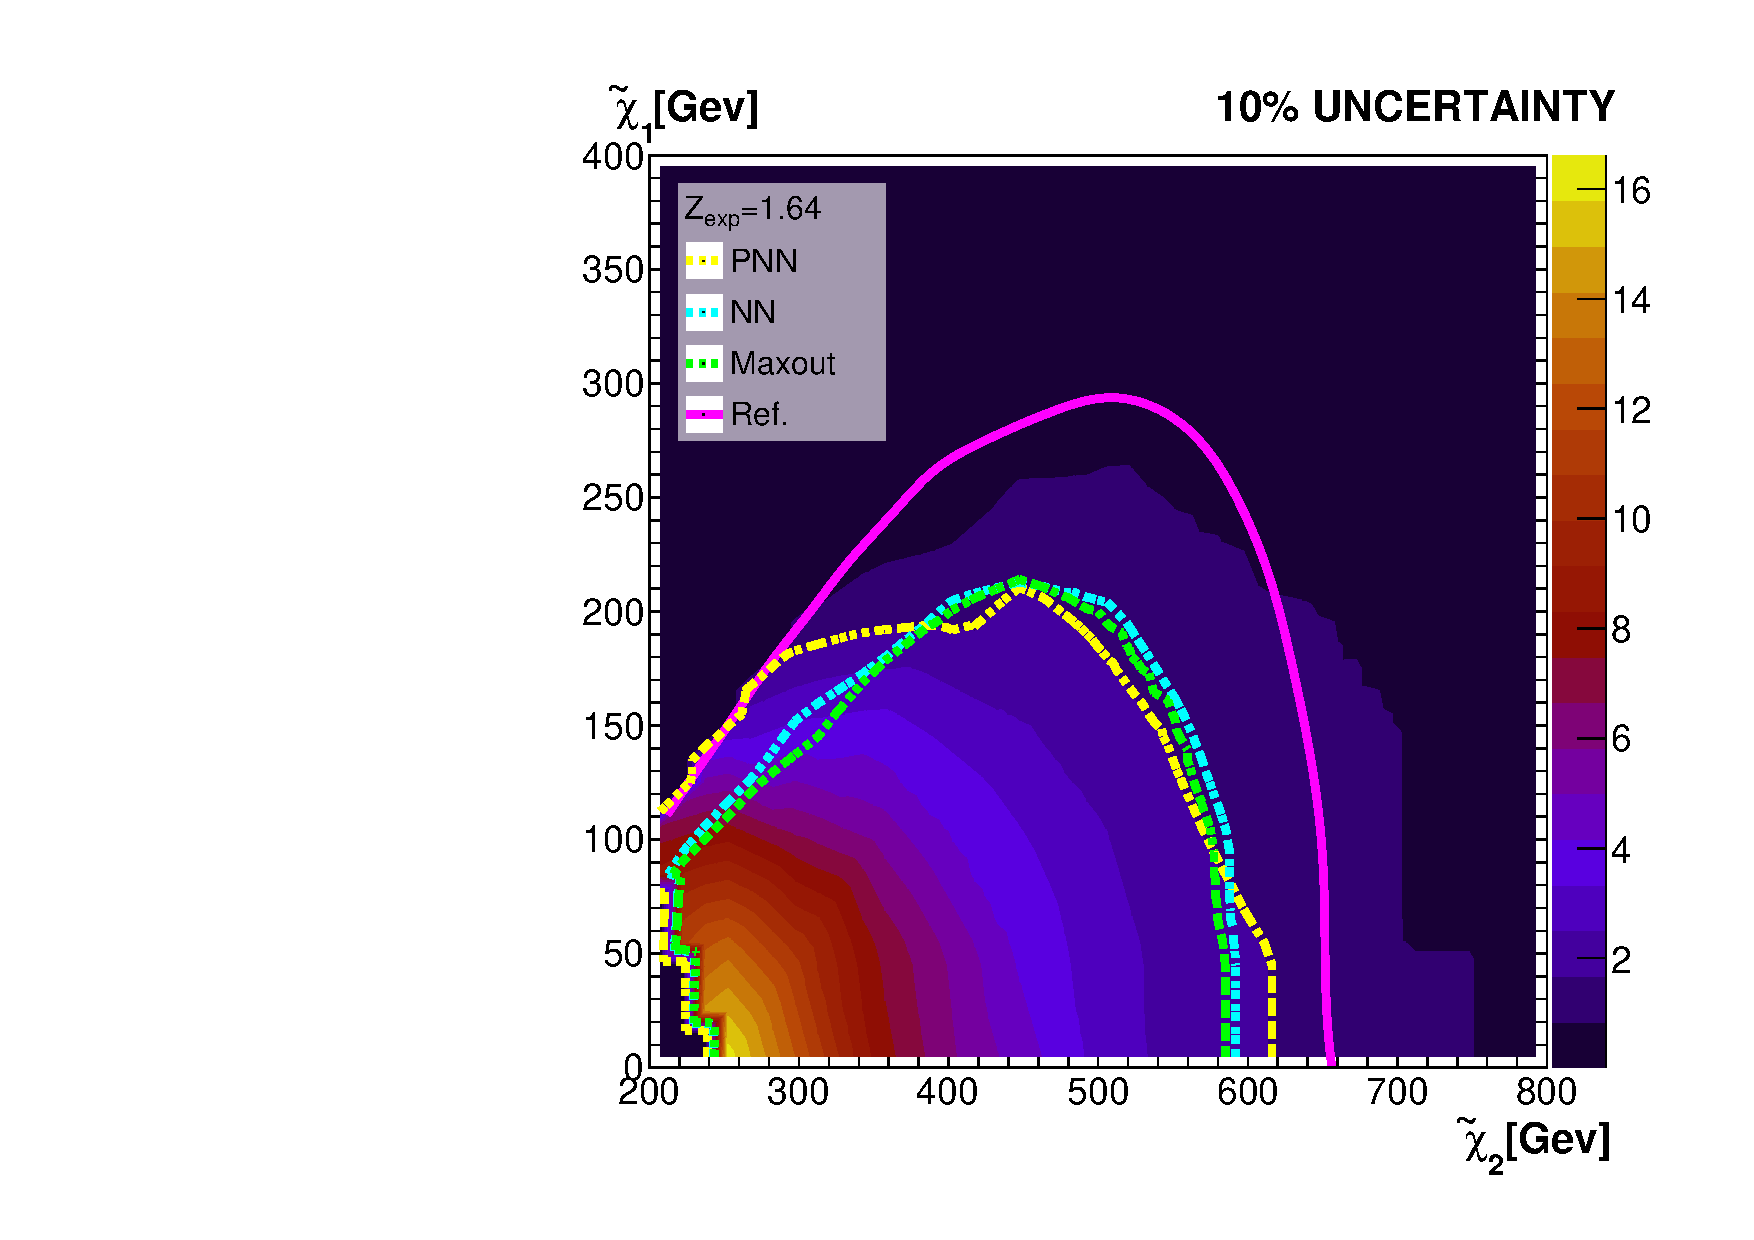
\includegraphics[width=0.45\textwidth]{figures/Limits/compLimit10.pdf}
    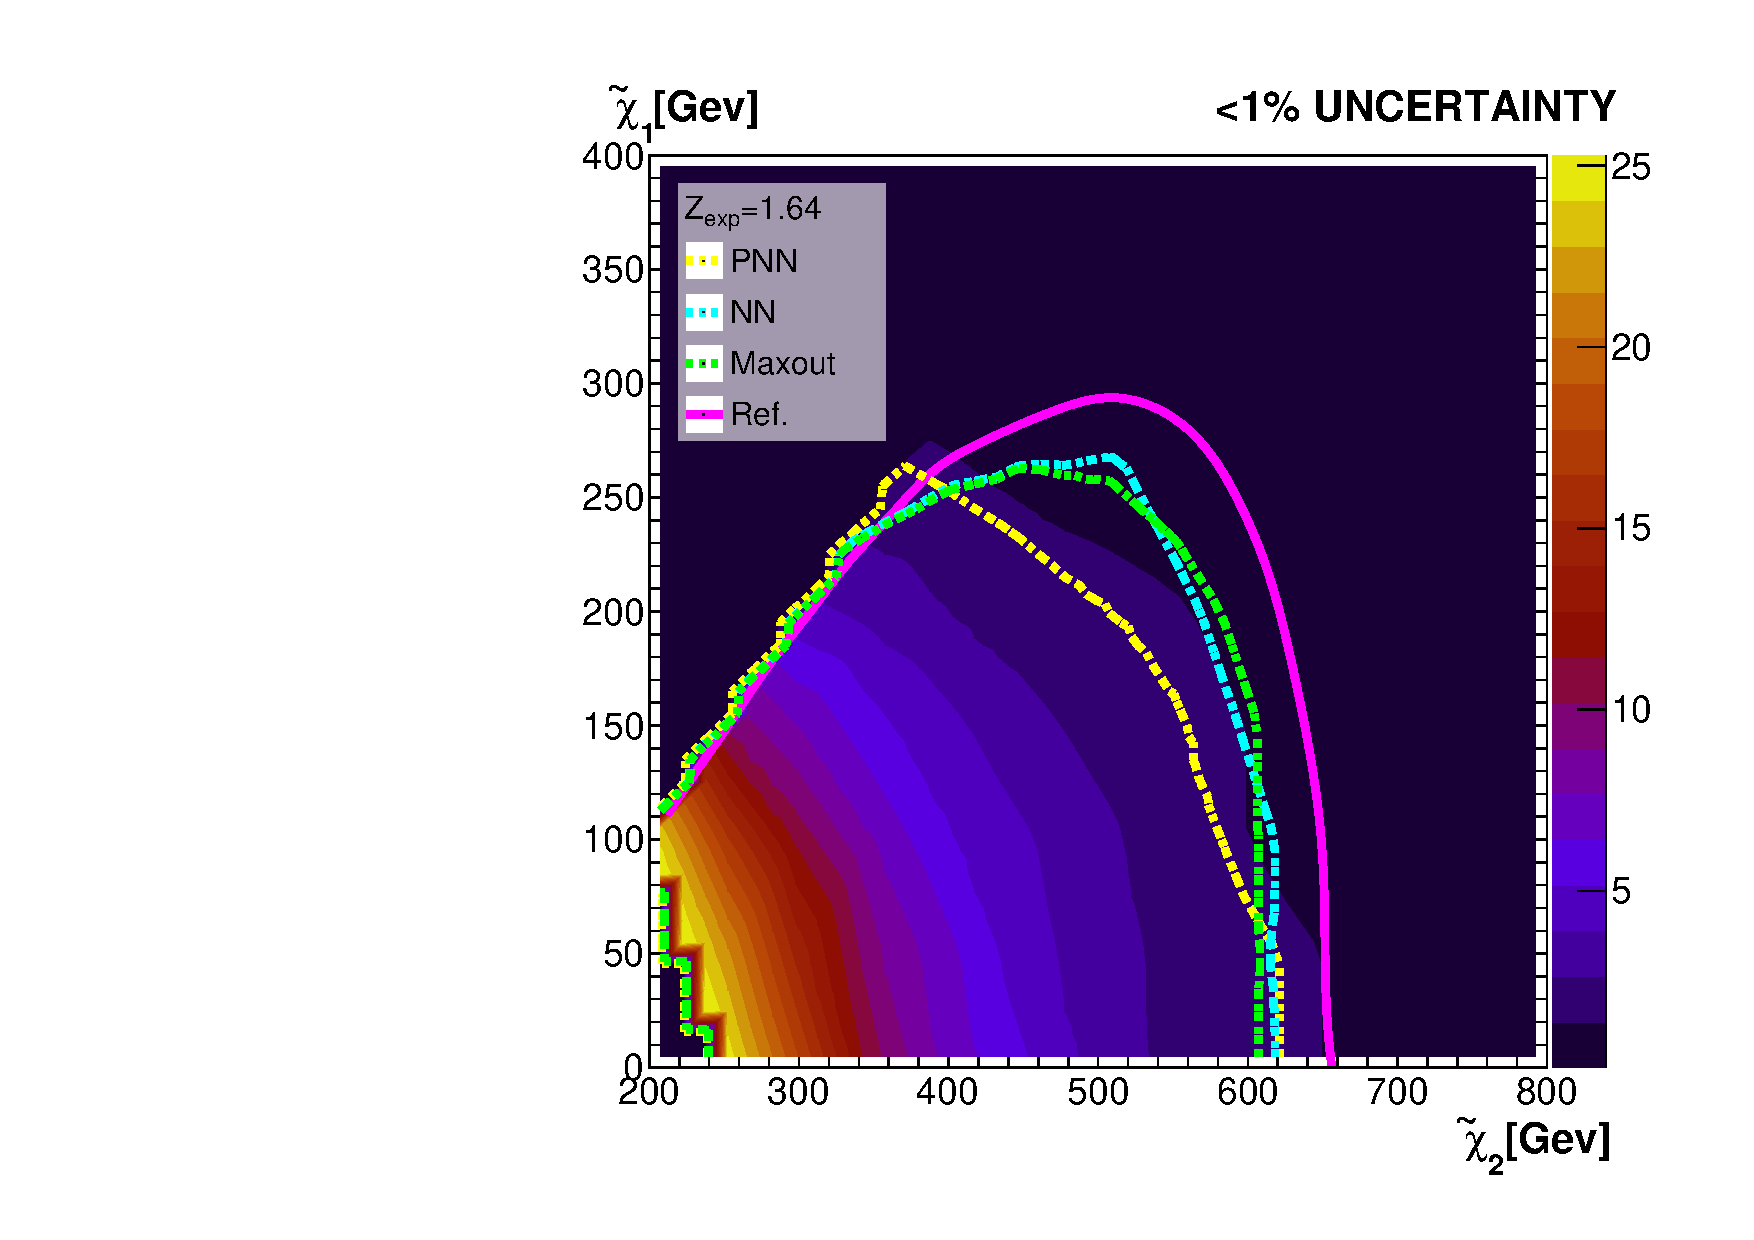
\includegraphics[width=0.45\textwidth]{figures/Limits/compLimit1.pdf}
    \begin{textblock}{1}(-0.32,.39)
        \tiny
        \cite{atlas_search_2021}
    \end{textblock}
    \begin{textblock}{1}(0.112,.39)
        \tiny
        \cite{atlas_search_2021}
    \end{textblock}
\end{frame}
\section{Conclusion $\&$ Outlook}
\begin{frame}{Outline}
    \tableofcontents[currentsection]
\end{frame}
\begin{frame}{Conclusion $\&$ Outlook}
    \begin{enumerate}
        \item Including a diverse signal set can improve performance
        \item The LWTA layers improve long-term memory via pattern specific pathways
        \item All network variants outperformed default settings of XGBoost
        \item PCA increased sensitivity of PNN and maxout model in original signal set
        \item None of the networks extended expected limit past previous ATLAS analysis
        \item PNN exhibited bias towards lower masses, whereas maxout model achieved a more balanced 
              sensitivity
        \item LWTA layer's increase in long-term memory is promising in future analysis 
              where higher masses are studied 
    \end{enumerate}
\end{frame}





\begin{frame}[allowframebreaks]{References}
    \begin{thebibliography}{}

        \bibitem{atlas_search_2021}
        ATLAS Collaboration.
        \newblock \enquote{Search for chargino--neutralino pair production in final states with three leptons and missing transverse momentum in {$\sqrt{s}$} = 13 {TeV} pp collisions with the {ATLAS} detector}.
        \newblock \url{http://arxiv.org/abs/2106.01676}


    \end{thebibliography}
\end{frame}


\end{document}